\pdfobjcompresslevel=0
\pdfcompresslevel=9
\pdfminorversion=7
\documentclass[letterpaper, 12, one column]{article}
%% packages %%

% === Rasterizar PDFs pesados automáticamente ===
\usepackage{graphicx,xifthen}
\newif\iffigdraft
% \figdrafttrue   % ← descomenta para compilar rápido (raster a 150 dpi)
% \figdraftfalse  % ← descomenta para calidad final (raster a 300 dpi)




\usepackage{tikz}
\usepackage{amsmath}

\usetikzlibrary{angles, quotes}

\usepackage{hyperref}
\usepackage{graphics,color}
\usepackage[table]{xcolor} 
\usepackage{tabularray}
\usepackage{epsfig} 
\usepackage{psfrag,epsfig}
\usepackage{graphics}                       % Soporte gráfico
\usepackage{changepage}
\usepackage{graphicx}   
\usetikzlibrary{arrows.meta}% Soport\e gráfico adicional
\usepackage{epstopdf}
\usepackage{float}
\usepackage{mathptmx} 
\usepackage{times} 
\usepackage{amsmath}
\usepackage{amssymb}  
\usepackage{booktabs}
\usepackage{bm}  
\usepackage{rotating} % <-- Asegúrate de incluir esto en el preámbulo
\usetikzlibrary{angles, quotes,shapes}
\usepackage{color}
\usepackage{multirow} 
\usepackage{cleveref}
\usepackage{cite}
% \usepackage{arydshln}  % Commented out - conflicts with longtable
\usepackage{tabularx}
\usepackage{booktabs}
\usepackage{microtype}
\usepackage{longtable}
\usepackage{lscape}
\usepackage{multirow}
\usepackage{array}
\usepackage{xcolor}
\usepackage{subcaption}
%\usepackage[caption=false]{subfig}
\usepackage{tikz}
    \usetikzlibrary{positioning,mindmap,arrows.meta,bending}
    \usetikzlibrary{mindmap, backgrounds, calc} % Mindmap drawing library 
    \usetikzlibrary{positioning,shapes,shadows,arrows, shapes.geometric}
\usepackage{adjustbox}
\newcommand{\gc}[1]{\textcolor[rgb]{1.00,0.00,0.00}{#1}}
\providecommand{\var}[1]{{\ensuremath{var}}\{#1\}}
\DeclareMathOperator{\tire}{\negthinspace-\negthinspace}
\DeclareRobustCommand{\legend}[1]{%
	\textcolor{#1}{\rule{1ex}{2ex}}%
}
\newcommand{\lineplot}[1]{
	\textcolor{#1}{\rule{1.5ex}{0.3ex}}%
}

%\setbeamertemplate{itemize/enumerate body begin}{\large}
%\usepackage{enumitem}
\newcommand{\tikzmark}[1]{\tikz[baseline,remember picture] \coordinate (#1) {};}

\usepackage{booktabs,colortbl,pifont}
\definecolor{completed}{RGB}{220,235,220}   % light green
\definecolor{writing}{RGB}{255,235,200}     % light orange
\newcommand{\cmark}{\ding{52}}   % ✔
\newcommand{\wmark}{\ding{118}}  % ⌘ (for “writing” phase) – choose any
\renewcommand{\arraystretch}{1.15}
%% commands %%
\DeclareMathAlphabet{\mathantt}{OT1}{antt}{li}{it}
\DeclareMathAlphabet{\mathpzc}{OT1}{pzc}{m}{it}
\providecommand{\abs}[1]{\lvert#1\rvert}
\providecommand{\norm}[1]{\lVert#1\rVert} 
\providecommand{\ppunto}[2]{\langle#1,#2\rangle}
\providecommand{\dist}[2]{{ d}(#1, #2)} 
\providecommand{\promed}[1]{{\fam=8 E}\{#1\}}
\providecommand{\cov}[2]{{\fam=7 cov}\{#1, #2\}}
\providecommand{\gaus}[2]{{\fam=6 N}(#1 #2)}
\providecommand{\unif}[1]{{\fam=6 U}(#1 )} 
\providecommand{\ve}[1]{{\bm {#1}}} 
\providecommand{\mat}[1]{{\bm {#1}}} 
\providecommand{\est}[1]{{\widetilde {#1}}}
\providecommand{\diag}[1]{{\rm{diag}}(#1)}
\newcommand{\jc}[1]{\textcolor[rgb]{0.00,0.0,1.00}{#1}}


\usepackage{longtable}
\usepackage{lscape}
\usepackage{multirow}
\usepackage{array}
\usepackage{xcolor}
\usepackage{xcolor}
\usepackage{soul}
\usetikzlibrary{positioning, arrows.meta}
%\usepackage{subcaption}

%\usepackage[hyperindex, colorlinks, citecolor=blue, linkcolor=blue, breaklinks=true, bookmarksopen]{hyperref}
\newcommand{\fou}{\ensuremath{\mathcal{F}}}%Para crear la F de Fourier
\newcommand{\ent}{\ensuremath{\mathbb{Z}}}%Pa crear algo parecido a la Z de enteros
\newcommand{\Z}{\ensuremath{\mathbb{Z}}}%Pa crear algo parecido a la R de reales
\newenvironment{definición}{\it \vspace{.4cm}\hrule \vspace{.2cm}}{\par\sf \vspace{.2cm}\rm\hrule\vspace{.4cm}}

%%%%%%%%%%%%%%%%%%%%%%%%%%%%%%% Custom Commands %%%%%%%%%%%%%%%%%%%%%%%%%%%%%%%%
\usepackage{tikz}
\usetikzlibrary{external}
\providecommand{\abs}[1]{\left| #1 \right|}
\providecommand{\norm}[1]{{\lVert #1 \rVert}_2}
\providecommand{\normH}[1]{{\lVert #1 \rVert}_\mathscr{H}}
\providecommand{\promedd}[2]{\mathbb{E}_{#1}\!\left\{#2\right\}}% op{\tiny }erador de promedio
\providecommand{\prodpunto}[2]{\left\langle #1,#2\right\rangle}

\providecommand{\paren}[1]{\!\left(\!#1\!\right)\!}
\newcommand{\T}{\top\!}
\newcommand{\p}{\prime\!}

\providecommand{\median}[1]{\text{median}\!\left(\!#1\!\right)}
\providecommand{\sign}[1]{\text{sign}\!\left(\!#1\!\right)}
\providecommand{\ve}[1]{{\bm{#1}}} %
\providecommand{\tr}[1]{{\operatorname{tr}\left({#1}\right)}}
\providecommand{\mat}[1]{{\bm{#1}}} %
\providecommand{\var}[1]{{\operatorname{var}}\left\{#1\right\}}
\providecommand{\map}[1]{\varphi\!\left(#1\right)}
\newcommand{\Real}{\mathbb{R}}
\newcommand{\N}{\mathbb{N}}
%\newcommand{\Z}{\mathbb{Z}}
\newcommand{\unos}{\ve{1}}
\providecommand{\kernel}[2]{\kappa\negthinspace\left(#1,\negthinspace#2\right)}
\DeclareMathOperator{\subconj}{\negthinspace\subset\negthinspace }
\DeclareMathOperator{\en}{\!\in\!}
\DeclareMathOperator{\igual}{\negthinspace=\negthinspace} 
\DeclareMathOperator{\diferente}{\negthinspace \neq \negthinspace}
% \DeclareMathOperator{\dist}{\operatorname{d}}

%\DeclareMathOperator{\xx}{\negthickspace\times\negthickspace}
\providecommand{\s}[1]{\negthinspace#1\negthinspace}%

\usepackage[normalem]{ulem}
%% Color text %%
\providecommand{\falta}[1]{\textcolor{green}{\underline{#1}}}
\providecommand{\duda}[1]{\textcolor{yellow}{{#1}}}
\providecommand{\am}[1]{\textcolor{green}{#1}}
\providecommand{\je}[1]{\textcolor{blue}{#1}}

% Note: pifont, \cmark and \xmark already defined at line 73-77
\definecolor{mypink1}{rgb}{0.858, 0.188, 0.478}
\usepackage{graphicx,xifthen,xstring} % <— necesario

\newif\iffigdraft
% \figdrafttrue   % ← modo rápido (150 dpi)
\figdraftfalse    % ← modo final (300 dpi)

\newcommand{\rasterpdffile}[3][]{%
  % Uso: \rasterpdffile[<dpi>]{ruta/figura.pdf}{<ancho>}
  \def\dpi{#1}%
  \ifthenelse{\isempty{#1}}{\iffigdraft\def\dpi{150}\else\def\dpi{300}\fi}{}%
  \StrBefore{#2}{.pdf}[\base]%
  \IfFileExists{\base.ras@\dpi.png}{}{%
    \immediate\write18{gs -q -dSAFER -dBATCH -dNOPAUSE -sDEVICE=pngalpha -r\dpi
      -dFirstPage=1 -dLastPage=1 -o "\base.ras@\dpi.png" "#2"}%
  }%
  \includegraphics[width=#3]{\base.ras@\dpi.png}%
}

 % {A multimodal deep learning approach with preserved interpretability to support remote sensing tasks}}

\title{Explainable Deep Learning Framework for Estimating and Generating Magnetic Domains from Hamiltonian Parameterss}
\author{\emph{PhD Thesis Proposal}\\ Juan Sebastián Méndez Rondón \\ \texttt{\small jumendezro@unal.edu.co} \\ \\ \\ 
Advisor: Prof. Andr\'es Marino \'Alvarez-Meza \\ \small{Universidad Nacional de Colombia - Sede Manizales} \\ \small{Facultad de Ingenier\'ia y Arquitectura} \\ \texttt{\scriptsize   amalvarezme@unal.edu.co} 
\\ \\ 
Co-Advisor: Prof. Jorge Ivan Montes\\ \small{Universidad Nacional de Colombia - Sede la paz}  \\ \texttt{\scriptsize  jimontesm@unal.edu.co } }

%Lack of interpretability
\date{Doctorado en Ingenier\'ia - Autom\'atica \\ Universidad Nacional de Colombia - Sede Manizales}
% ====== PREÁMBULO COMPATIBLE CON TUS TABLAS ======
\usepackage{booktabs,tabularx,array,changepage,float}
\usepackage{soul,xcolor}
\sethlcolor{yellow!20}

% Macros de ancho usadas por tus tablas
\newlength{\fulllength}  \setlength{\fulllength}{\textwidth}
\newlength{\extralength} \setlength{\extralength}{0pt}

% Columna centrada expandible "C" para tabularx
\newcolumntype{C}{>{\centering\arraybackslash}X}


\begin{document}
\maketitle
\section{Abstract}
The study of magnetic domain structures in nanoscale materials is essential for advancing
emerging technologies in spintronics, biomedicine, and energy storage \cite{Wang2022, Rarokar2024, Lak2021}. 
Magnetic nanoparticles and nanodots exhibit complex spin textures—such as vortices, skyrmions,
and stripe domains—that determine their functional behavior in applications ranging from magnetic
memory bits to targeted hyperthermia \cite{Wang2022, Lak2021, Zelent2021}. Understanding and controlling
these states requires a deep connection between the parameters of the magnetic Hamiltonian
(exchange, anisotropy, Dzyaloshinskii–Moriya interaction, external field, and temperature) and the
resulting spatial spin configurations \cite{Zelent2021, Ga2022, Fert2023}.

However, several fundamental challenges persist at the nanoscale. The first is the nonlinearity and
high dimensionality of the mapping between physical parameters and domain patterns, which prevents
direct analytical inversion \cite{WangMicromag2024, DeepMLHam2024}. The second is degeneracy:
distinct combinations of Hamiltonian parameters can yield visually similar configurations, complicating
inverse identification \cite{Feng2024, Liu2023}. Third, experimental limitations—such as noise, finite
probe resolution, tip–sample convolution in MFM, and sample variability—hinder quantitative
interpretation of MFM or SP-STM images \cite{Makarova2022, Bagchi2024}. Finally, the computational cost
of atomistic or micromagnetic simulations restricts large-scale parameter sweeps, limiting predictive
exploration of material regimes \cite{WangMicromag2024, MuMax3docs}.

Deep learning has emerged as a powerful tool to bridge this gap. The inverse problem—inferring
physical parameters from magnetic domain images—has been successfully addressed using CNNs and
explainable regression frameworks \cite{Kong2023, AIP2022, DeepMLHam2024}. The direct problem—
generating domain configurations from parameters—has been explored in materials science using
generative models such as VAEs and conditional GANs \cite{MicroVAE2023, Ronne2024}. These methods
can reproduce general morphologies but suffer from poor interpretability, instability under noise, limited
generalization, and lack of physical constraints \cite{Feng2024, Park2024, MicroVAE2023}.


% AGREGAR EL PARRAFO INTRODUCTORIO ASOCIADO A LAS TAREAS QUE SE VAN A GENERAR. -- > REVISAR CON ANDRES MARINO.

%% FIGURA DEL PROBLEMA INVERSO Y DIRECTO --CHECK

%% CAMBIAR EL PROBLEMA MIXTO DEGENERAY OF CONFIGURATIONS --CHECK
%% 2 parrafos uno que conceptualmente explique que es  y las posibles causas segun la fisica. --CHECK
%% LOW QUALITY DATA. 

%% explicabilidad fisica.
%% RESUMIR EN UNA TABLA O DIBUJO EL ESTADO DEL ARTE.
%% tabla con items para los proyectos futuros.




% TUTORIAL DE REDES INFORMADAS POR LA FISICA -- MIRAR COMO LLEVARLO A UN METODOLOGIA DE OPTIMAZCIÓN BAYESIANA. - QUE SEA EXPLICABLE. COMO PUEDO SINTONIZAR DICHOS CON INTERPRETABILIDAD.
%% CON UN EJERCICIO BASICO.


Recently, diffusion-based models have achieved state-of-the-art performance in conditional image
synthesis and inverse design across materials science \cite{Alverson2024, Chen2024, SyMat2023}. Yet,
their application to magnetic systems remains underexplored, and existing generative strategies rarely
enforce physical consistency—such as energy minimization or Hamiltonian symmetry—limiting their use
for predictive materials discovery \cite{Ronne2024, Park2024}.


This work proposes a unified deep learning framework for the direct and inverse estimation of magnetic Hamiltonian parameters and nanoscale domain configurations. Instead of relying on a fixed generative architecture, the framework will explore families of regularized and variational deep learning methodologies capable of integrating physical priors—such as Hamiltonian constraints, energy-based consistency, or symmetry-aware embeddings—to enhance robustness under degeneracy and low-quality data conditions. \cite{Sparks2024, Optuna2022}.


\section{Motivation}

%1.1. Contexto general: el magnetismo a nanoescala

The study of magnetic systems at the nanoscale has gained strategic importance in
modern materials science \cite{Wang2022, Lak2021}. In particular, magnetic nanoparticles (MNPs) and nanodots
constitute platforms where spin interactions and collective quantum properties give
rise to emergent phenomena of great scientific and technological interest \cite{Jiang2023, Rarokar2024}. At these
scales, the balance between exchange interactions, anisotropy, Dzyaloshinskii–Moriya
interaction (DMI), and external magnetic fields generates a wide variety of magnetic
textures—vortices, skyrmions, helical domains, and labyrinthine configurations \cite{Ga2022, Fert2023, Tokura2021}. These
structures determine the magnetic response, thermal stability, and switching dynamics
of the material, which are key aspects for functionality in advanced devices \cite{Song2023, Wang2022}.


\begin{figure}[H]
    \centering
    \includegraphics[width=0.75\textwidth]{Figures/magneticTexture.jpg}
    \caption{ Magnetic domains configurations }
    \label{fig:skyrmions_textures}
\end{figure}

%1.2. Relevancia aplicada: por qué las nanopartículas magnéticas importan

Magnetic nanoparticles and nanodots possess a unique versatility that makes them
relevant across multiple fields:  
a) Spintronics and Non-Volatile Magnetic Memories. Topologically protected magnetic textures, such as skyrmions, enable the storage of information as stable and switchable bits. These structures support the development of MRAM, racetrack memories, and magnetic logic devices, combining high density, low power consumption, and radiation resistance \cite{Morshed2021, Sisodia2022, Zhang2015, Eurek2024}.


\begin{figure}[H]
    \centering
    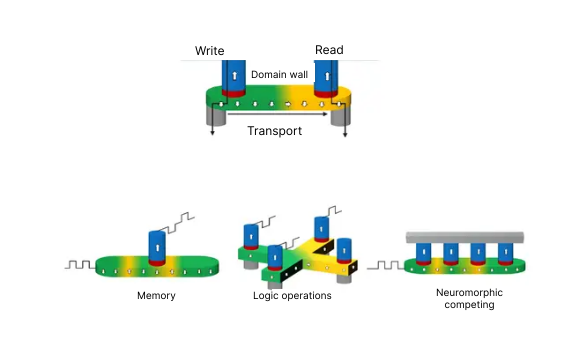
\includegraphics[width=0.75\textwidth]{Figures/mram.png}
    \caption{ Magnetic Random Memories }
    \label{fig:skyrmions_textures}
\end{figure}


b) Magnetic nanoparticles are used in oncological hyperthermia therapies, drug targeting, and enhanced magnetic resonance imaging (MRI). Their efficiency depends on the dynamic spin response under alternating fields, which is determined by the internal structure and anisotropy of the material \cite{Barrera2023, IronOxideReview2023, MLDesign2023}.


\begin{figure}[H]
    \centering
    \includegraphics[width=0.75\textwidth]{Figures/medicine.jpg}
    \caption{ Biomedical applications }
    \label{fig:skyrmions_textures}
\end{figure}

c) Energy Conversion and Storage. In the energy field, magnetic nanoparticles are
investigated for magnetocaloric refrigeration, thermoelectric conversion, and magnetic
energy storage \cite{He2025, Nehan2024, Hadouch2022}. The spin configurations determine
the mechanisms of energy transfer between magnetic and thermal degrees of freedom,
directly influencing the efficiency of these processes \cite{Liedienov2021, Nehan2024}.


\begin{figure}[H]
    \centering
    \includegraphics[width=0.45\textwidth]{Figures/storage.png}
    \caption{ Biomedical applications }
    \label{fig:skyrmions_textures}
\end{figure}





%2.4 Scientific Importance of Nanoscale Studies

The analysis of magnetic systems at the nanoscale not only drives the development of new technologies but also contributes fundamental knowledge about emergent phenomena in condensed matter physics \cite{Xiao2023, Liao2023}. These systems serve as natural models of complex physical behavior, where local interactions give rise to collective responses that challenge classical linear approximations \cite{Xiao2023, DeepSPIN2023}.

In recent years, the integration of Artificial Intelligence (AI) with computational physics has opened new avenues for the modeling and prediction of complex material behaviors \cite{Hilgers2025, Ryu2025, Goswami2022}. Traditional simulation methods offer precise control over physical parameters but are limited by high computational cost and restricted scalability across parameter spaces \cite{Liao2023}. AI-driven approaches, particularly deep learning architectures, enable the extraction of latent physical relationships directly from data, accelerating the exploration of vast configuration spaces that would otherwise be computationally intractable \cite{Xiao2023, Hilgers2025}. When coupled with physics-informed principles, these models not only enhance predictive accuracy but also preserve interpretability and physical consistency \cite{Ryu2025, Sharma2023}. In the context of nanoscale magnetism, such hybrid frameworks bridge the gap between experimental observation and theoretical modeling, providing a data-efficient path toward inverse design and the discovery of emergent spin phenomena \cite{DeepSPIN2023, Liao2023}.


\vspace{0.5cm}
%%% PARRAFO CON RELACIÓN A GCPDS
%%%
%%% REFERENCIAS DEL GRUPO?
%%%
This work is developed within the Research Signal Processing and Recognition  (GCPDS), which has extensive experience in the design and implementation of intelligent systems for signal and image analysis. The group has explored artificial intelligence methodologies across multiple domains, including image processing, temporal series analysis, and, more recently, electroencephalographic (EEG) signal interpretation. Building on this background, GCPDS is currently expanding its research toward the application of AI in computational physics, focusing on the intersection between data-driven learning and physical modeling. Current efforts involve the integration of generative models, interpretability mechanisms, transformer-based architectures, and optimization strategies to develop hybrid frameworks capable of revealing underlying physical principles from complex experimental data. This interdisciplinary approach establishes a foundation for applying advanced machine learning to the understanding and design of magnetic systems at the nanoscale. %% PAULINA


\section{Problem Statement}
%%%% Experimental and Theoretical Approaches to Magnetic Nanostructures
 
The study of magnetic nanostructures integrates two complementary approaches: the \textbf{experimental} and the \textbf{theoretical-simulation} pathways \cite{Streubel2022}. The experimental route focuses on the physical synthesis, visualization, and measurement of magnetic systems \cite{Zhang2024MFM, Wiesendanger2022SPSTM}, whereas the theoretical approach aims to model and predict their magnetic behavior from first principles or phenomenological descriptions \cite{Evans2014Atomistic, MuMaxReview2021}.


From the experimental perspective, research begins with the \textit{sample preparation} of thin films, multilayers, or nanostructures that define the system’s geometry and magnetic anisotropy \cite{Nagaosa2021Deposition, Fert2022ThinFilms}. These samples are then characterized through advanced \textit{magnetic imaging techniques} such as Lorentz Transmission Electron Microscopy (TEM), Magnetic Force Microscopy (MFM), and Kerr microscopy, which reveal the domain patterns at nanometer resolution \cite{Streubel2022, Zhang2024MFM, McVitie2023Lorentz}. The resulting data are complemented by \textit{acquisition and analysis} of external stimuli, including magnetic and electric fields (STT and SOT effects), strain fields, and temperature variations, which allow for the control and manipulation of domain structures \cite{Manchon2019SOT, Yu2022StrainControl, Finco2024Stimuli}.


In parallel, the theoretical and computational approach seeks to describe these systems at different scales. At the \textit{atomistic level}, models such as the Heisenberg Hamiltonian and Monte Carlo simulations capture spin interactions with atomic precision \cite{Evans2014Atomistic, Nowak2007MC, Hinzke2022Atomistic}. Moving to larger scales, \textit{micromagnetic simulations} employ the Landau–Lifshitz–Gilbert (LLG) equation to model the continuous magnetization field, implemented through frameworks like MuMax3, OOMMF, and Spirit \cite{MuMaxReview2021, Donahue1999OOMMF, Spirit2020}.

Together, these methodologies constitute a multi-scale, multi-modal ecosystem that bridges empirical observation and theoretical understanding, providing the foundation for modern research in magnetic materials \cite{Gomez2023MultiscaleReview}.



\begin{figure}[H]
    \centering
    \includegraphics[width=0.75\textwidth]{Figures/ProblemStatement.png}
    \caption{ Magnetic Domain Approach }
    \label{fig:skyrmions_textures}
\end{figure}

From an experimental perspective, advances in Magnetic Force Microscopy (MFM) and Spin-Polarized Scanning Tunneling Microscopy (SP-STM) have enabled direct visualization of nanoscale magnetic textures, revealing complex domain morphologies such as vortices, skyrmions, and labyrinthine patterns \cite{Zhang2024MFM, Wiesendanger2022SPSTM, McVitie2023Lorentz}. However, experimental images often contain noise, contrast distortions, and limited resolution, making quantitative parameter extraction challenging \cite{Gao2021NoiseMFM, Phark2022ResolutionLimits}. As a result, bridging the gap between simulated and observed magnetic configurations remains an open problem that hinders both predictive modeling and materials discovery \cite{Liao2023, DeepSPIN2023, Finco2024Stimuli}.


%%%%%%%%%%%%%%%%%%%%%%%%%%%%%%%%%%%%%%%%%%%%%%%%%%%%%%%%%%
%%% EXTENSIÓN PARA HABLAR DE LAS SIMULACIONES Y PROBLEMAS 
%%%%%%%%%%%%%%%%%%%%%%%%%%%%%%%%%%%%%%%%%%%%%%%%%%%%%%%%%%
Despite the significant advances in atomistic and micromagnetic simulations, the theoretical–computational approach faces several inherent limitations that restrict its scalability and practical applicability. First, the computational cost associated with solving high-dimensional Hamiltonian systems grows rapidly with the number of spins and spatial resolution, making large-scale or time-dependent studies computationally prohibitive \cite{Gomes2022Limitations, Hinzke2022Atomistic}. Parameter sweeps over exchange coupling, anisotropy, or Dzyaloshinskii–Moriya interaction (DMI) often require thousands of independent simulation runs, each demanding considerable processing time and memory resources \cite{Gomez2023MultiscaleReview, MuMaxReview2021}, and the approximation level of each simulation method imposes constraints on physical fidelity \cite{Nowak2007MC, Evans2014Atomistic}. Atomistic models offer high precision but are limited to small systems, while micromagnetic models extend spatial coverage at the expense of losing atomistic detail \cite{Spirit2020, McMichael2009Limitations}. Incorporating temperature effects, stochastic fluctuations, and material imperfections further increases complexity and reduces interpretability \cite{Hinzke2022Atomistic, Brown1963Thermal}.  



%%%%%%%%%%%%%%%%%%%%%%%%%%%%%%%%%%%%%%%%%%%%%%
% INTRODUCCIÓN AL PROBLEMA INVERSO Y DIRECTO %
%%%%%%%%%%%%%%%%%%%%%%%%%%%%%%%%%%%%%%%%%%%%%%
Within this integrated context, the study of magnetic nanostructures can be framed around two complementary and interdependent challenges: the direct and the inverse magnetic domain problems \cite{Feng2024, Liao2023}.

The direct problem involves predicting or generating the magnetic domain configuration that emerges from a given set of Hamiltonian parameters—exchange interaction, anisotropy, DMI, external magnetic field, and temperature. This process defines the forward mapping from the parameter space to the spatial magnetization distribution and is typically addressed using micromagnetic or atomistic simulations \cite{Evans2014Atomistic, MuMaxReview2021, Nowak2007MC}. However, such simulations are often computationally intractable for broad parameter exploration or for incorporating stochastic thermal and experimental effects \cite{Gomes2022Limitations, Hinzke2022Atomistic, Brown1963Thermal}.


\begin{figure}[H]
    \centering
    \includegraphics[width=0.75\textwidth]{Figures/Direct.png}
    \caption{ Magnetic Domain Approach }
    \label{fig:skyrmions_textures}
\end{figure}

In contrast, the inverse problem aims to infer the underlying physical parameters responsible for a given observed domain configuration, such as those obtained from Magnetic Force Microscopy (MFM) or Spin-Polarized Scanning Tunneling Microscopy (SP-STM) \cite{Zhang2024MFM, Wiesendanger2022SPSTM}. This task is intrinsically ill-posed: multiple parameter combinations can reproduce visually similar textures, leading to degeneracy and uncertainty in parameter estimation \cite{Feng2024, Liu2023, DeepSPIN2023}.


\begin{figure}[H]
    \centering
    \includegraphics[width=0.75\textwidth]{Figures/Inverse.png}
    \caption{ Magnetic Domain Approach }
    \label{fig:skyrmions_textures}
\end{figure}

Bridging these two directions—ensuring coherence between generation (direct mapping) and estimation (inverse mapping)—is essential for predictive materials discovery \cite{Feng2024, Park2024}. A unified and physically consistent framework that can simultaneously learn both directions offers a pathway toward explainable, data-driven modeling of nanoscale magnetic phenomena \cite{DeepSPIN2023, Ryu2025, Hilgers2025}.

Overall, the study of magnetic nanodots is constrained by three fundamental challenges that motivate the development of hybrid approaches combining physical modeling and data-driven inference \cite{Gomez2023MultiscaleReview, Liao2023, Evans2014Atomistic}.



\begin{figure}[H]
\centering
\begin{adjustbox}{center, max width=\textwidth}
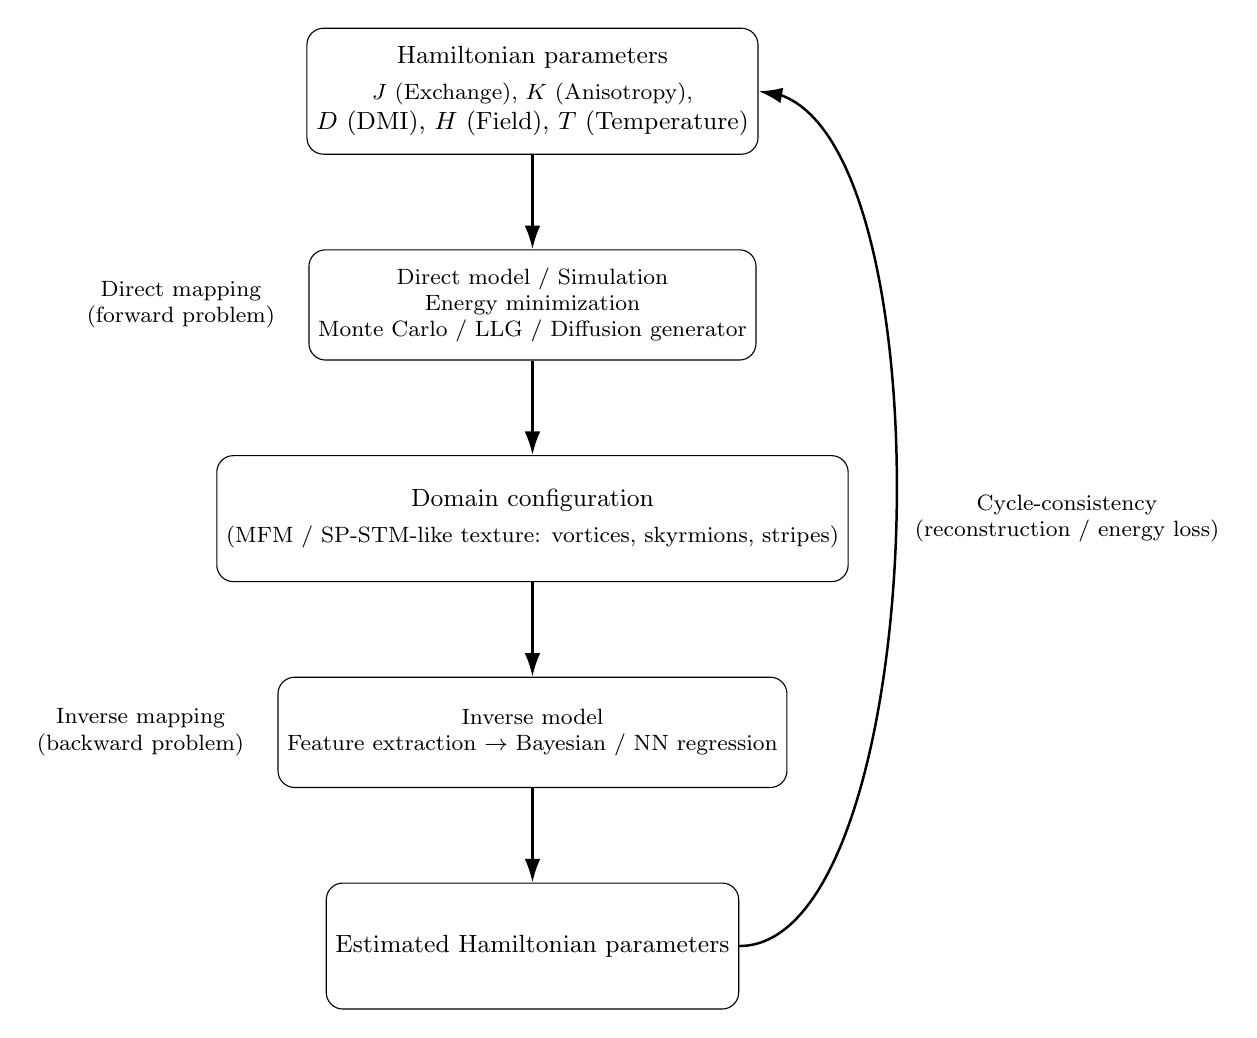
\begin{tikzpicture}[
  box/.style = {draw, rounded corners=6pt, minimum width=5cm, minimum height=1.6cm, align=center, font=\small},
  process/.style = {draw, rounded corners=6pt, minimum width=5cm, minimum height=1.4cm, align=center, font=\footnotesize},
  arr/.style = {-{Latex[length=3mm,width=2mm]}, line width=0.9pt},
  dashedarr/.style = {->, dashed, line width=0.9pt},
  node distance=12mm
]

% --- Nodes (top to bottom) ---
\node[box] (ham) {Hamiltonian parameters\\[2pt]
\footnotesize $J$ (Exchange), $K$ (Anisotropy),\\ $D$ (DMI), $H$ (Field), $T$ (Temperature)};

\node[process, below=of ham] (direct) {Direct model / Simulation\\
\footnotesize Energy minimization \\ Monte Carlo / LLG / Diffusion generator};

\node[box, below=of direct] (domain) {Domain configuration\\[2pt]
\footnotesize (MFM / SP-STM-like texture: vortices, skyrmions, stripes)};

\node[process, below=of domain] (inverse) {Inverse model \\ \footnotesize Feature extraction $\rightarrow$ Bayesian / NN regression};

\node[box, below=of inverse] (est) {Estimated Hamiltonian parameters};

% --- Arrows ---
\draw[arr] (ham) -- (direct);
\draw[arr] (direct) -- (domain);
\draw[arr] (domain) -- (inverse);
\draw[arr] (inverse) -- (est);

% --- Loop arrow back up (cycle consistency) ---
\draw[arr] (est.east) .. controls +(2.5,0) and +(2.5,0) .. (ham.east)
node[midway, right=1mm, font=\footnotesize, align=center] {Cycle-consistency\\(reconstruction / energy loss)};

% --- Labels ---
\node[font=\footnotesize, align=center, left=3mm of direct] {Direct mapping\\(forward problem)};
\node[font=\footnotesize, align=center, left=3mm of inverse] {Inverse mapping\\(backward problem)};

\end{tikzpicture}
\end{adjustbox}
\caption{Vertical unified cycle illustrating the direct (top-down) and inverse (bottom-up) problems in magnetic domain research. The cycle-consistency loop (right) enforces physical coherence between estimated Hamiltonian parameters and generated magnetic textures.}
\label{fig:vertical-cycle}
\end{figure}



Overall, the study of magnetic nanodots is constrained by three fundamental challenges that motivate the development of hybrid approaches combining physical modeling and data-driven inference:

\vspace{0.5cm}

\subsection{Degeneracy of Magnetic States}


\vspace{0.5cm}

Different combinations of Hamiltonian parameters—such as exchange interaction, anisotropy, and Dzyaloshinskii–Moriya interaction (DMI)—can lead to visually similar magnetic patterns \cite{Feng2024, Liao2023, DeepSPIN2023}. This degeneracy complicates the unique identification of physical parameters from experimental observations, creating ambiguity in inverse estimation tasks \cite{Park2024, Liu2023InverseML, Raju2022SkyrmionInverse}.


\begin{figure}[H]
    \centering
    \includegraphics[width=0.45\textwidth]{Figures/Problems1.png}
    \caption{Degenerate magnetic states arising from distinct parameter combinations.}
    \label{fig:degeneracy_problem}
\end{figure}

In nanoscale magnetic systems, the relationship between the Hamiltonian parameters and the resulting domain configurations is highly nonlinear and often degenerate \cite{Feng2024, Liao2023}. This degeneracy arises because different combinations of exchange coupling (J), magnetic anisotropy (K), and Dzyaloshinskii–Moriya interaction (D) can produce equilibrium states with similar total energy and comparable spatial magnetization patterns \cite{Raju2022SkyrmionInverse, DeepSPIN2023}. From a physical perspective, the energy landscape of the magnetic Hamiltonian contains multiple local minima corresponding to metastable spin textures—such as vortices, skyrmions, or labyrinthine domains—that can be stabilized under different parameter sets \cite{Leonov2020EnergyLandscape, Du2022MetaStableSkyrmions}. In practice, this means that small compensations between parameters can preserve the overall balance of competing interactions: for example, an increase in anisotropy can be offset by a stronger exchange term or a weaker DMI, yielding morphologically indistinguishable configurations \cite{Liu2023InverseML, Bessarab2018EnergyBarriers}. Thermal fluctuations and boundary effects further blur these distinctions by allowing transitions between nearby minima, effectively broadening the range of parameter combinations that generate similar observable textures \cite{Hertel2023Thermal, Maletta2021BoundaryEffects}. As a result, the mapping from physical parameters to domain patterns is non-injective, complicating the inverse identification of Hamiltonian parameters from experimental images and introducing intrinsic ambiguity in inverse modeling tasks \cite{Park2024, Ryu2025}.


\begin{figure}[H]
    \centering
    \includegraphics[width=0.8\textwidth]{Figures/NonUniqueness.png}
    \caption{Energy Landscape of magnetic hamiltonian}
    \label{fig:degeneracy_problem}
\end{figure}

In addition to energy-based degeneracy, a second source of non-uniqueness stems from the geometric symmetries intrinsic to many spin Hamiltonians. For systems where the magnetic energy is invariant (or nearly invariant) under in-plane rotations and translations, distinct domain configurations obtained by rotating or shifting the spin texture may represent the same physical state. Recent works exploiting equivariant neural-network architectures have shown that incorporating these Euclidean symmetries (rotational and translational) into the learning model significantly improves generalization and ensures physically consistent predictions across symmetry-related configurations \cite{Zhong2023EquivariantMagnetic, Yuan2024MagNet}. Consequently, image-based states differing only by rigid motions should be considered equivalent under the symmetry group, adding a geometric layer to the degeneracy beyond parameter compensation.


For data-driven approaches to forward (parameters → texture) or inverse (texture → parameters) mapping, neglecting geometric degeneracy can lead to spurious variability: models may reproduce correct energies but output textures that are rotated or translated versions of the 'reference', or misassign parameters to physically equivalent but geometrically different inputs. Equivariant models (i.e., models whose architecture respects the underlying symmetry group) or preprocessing steps that canonicalize orientation/position of textures have been demonstrated to significantly reduce such artifacts while preserving physical fidelity \cite{Miyazaki2023EquivariantSpinNN, Zhong2023EquivariantMagnetic}. Therefore, explicitly accounting for geometric symmetries is crucial to disentangle true degeneracy in parameters from trivial degeneracy due to spatial transformations.

\begin{figure}[H]
    \centering
    \includegraphics[width=0.8\textwidth]{Figures/GeometricDegeneracy.png}
    \caption{Geometric Degeneracy Effect}
    \label{fig:degeneracy_problem}
\end{figure}

\subsection{Low Quality Data}
Magnetic domain imaging and modeling face intrinsic limitations that affect the quality
and reliability of observable data. On the experimental side, characterization techniques
such as Magnetic Force Microscopy (MFM) and Spin-Polarized Scanning Tunneling
Microscopy (SP-STM) provide direct access to nanoscale magnetic textures but are
fundamentally constrained by instrumental noise, finite probe resolution, and contrast
distortions \cite{Schlenhoff2022SPSTM, Kramer2021MFMNoise, Raabe2020ImagingLimits}. These imperfections obscure the fine spatial structure of the magnetization
field, complicating the quantitative extraction of physical parameters and domain wall
profiles \cite{Hanneken2022ResolutionLimit, Wiesendanger2023SPSTMReview}. On the computational side, numerical simulations—whether atomistic or
micromagnetic—introduce their own forms of degradation. Discretization errors in
the mesh, finite time-step integration of the Landau–Lifshitz–Gilbert (LLG) dynamics,
and simplifications in boundary or anisotropy conditions limit the accuracy of the
resulting spin configurations \cite{Evans2014Atomistic, Exl2021NumericalErrors, Hertel2022MicromagneticLimits}. As a result, both experimental and simulated datasets
often represent only approximations of the true magnetic state, making the comparison
between observed and modeled textures inherently uncertain \cite{Liao2023, Park2024}.


\begin{figure}[H]
    \centering
    \includegraphics[width=0.45\textwidth]{Figures/Lab.png}
    \caption{Experimental observation limitations due to noise and resolution constraints.}
    \label{fig:experimental_limitations}
\end{figure}

\begin{table}[H]
\centering
\caption{Approximate operational costs and limitations of magnetic imaging techniques.}
\label{tab:experimental_costs_monetary}
\renewcommand{\arraystretch}{2}
\large
\resizebox{\textwidth}{!}{
\begin{tabular}{lcccc}
\hline
\textbf{Technique} & \textbf{Spatial Resolution} & \textbf{Main Limitations} & \textbf{Quantitative Accuracy} & \textbf{Estimated Cost (USD/hour)} \\ \hline
Magnetic Force Microscopy (MFM) & 30–50 nm & Tip-induced artifacts, long scan time & Moderate & 150–300 \\
Spin-Polarized STM (SP-STM) & $\sim$1 nm & Requires UHV and cryogenic conditions & High (atomic-level) & 800–1500 \\
Lorentz Transmission Electron Microscopy (Lorentz TEM) & 5–10 nm & Complex sample prep, projection effects & Moderate–High & 400–800 \\
Kerr Microscopy & 300–500 nm & Optical diffraction limit, surface sensitivity & Low–Moderate & 100–250 \\
X-ray Magnetic Circular Dichroism (XMCD) & 10–30 nm & Requires synchrotron access & High & 2000–5000 \\
Electron Holography & 2–5 nm & High vacuum, phase noise & High & 500–1000 \\ \hline
\end{tabular}
}
\end{table}


From a physical standpoint, this degradation is a direct manifestation of the multi-
scale and metastable nature of magnetic systems. The magnetic free-energy landscape
is rugged, containing multiple nearby minima separated by small energy barriers \cite{Leonov2020EnergyLandscape, Bessarab2018EnergyBarriers}. Even
slight variations in temperature, defects, or external fields can cause the system to
relax into different local minima that are energetically similar but structurally distinct \cite{Du2022MetaStableSkyrmions, Hertel2023Thermal}. Consequently, any measurement or simulation captures only one realization of a broader
ensemble of possible states. In experimental observations, this variability is further
blurred by the indirect nature of detection: instruments like MFM record the stray field
above the surface, which is a convolution of the probe’s sensitivity and the sample’s
magnetization, rather than a direct mapping of the spin structure itself \cite{Kramer2021MFMNoise, Raabe2020ImagingLimits}. Similarly, in
simulations, numerical smoothing and discretization coarsen the magnetization field,
suppressing high-frequency details \cite{Exl2021NumericalErrors, Hertel2022MicromagneticLimits}. Together, these effects impose a fundamental limit
on the fidelity of both experimental and computational data, constraining the precision
of parameter estimation and the interpretability of magnetic textures \cite{Liao2023, Park2024}.



\begin{figure}[H]
    \centering
    \includegraphics[width=0.97\textwidth]{Figures/Sensitive.png}
    \caption{Experimental observation limitations due to noise and resolution constraints.}
    \label{fig:experimental_limitations}
\end{figure}

\subsection{Lack of physic-based interpretability}
A persistent challenge in data-driven modeling of magnetic systems is the lack of in-
terpretability and physical traceability in the results. While modern machine learning
methods can efficiently approximate the complex mapping between Hamiltonian pa-
rameters and magnetic domain configurations, their internal representations are often
opaque, providing limited insight into the underlying physics that govern the observed
phenomena \cite{Rao2022ExplainableMaterialsML, Park2024, DeepSPIN2023}. This opacity complicates the validation of learned relationships against es-
tablished physical laws, such as exchange symmetry, anisotropy effects, or DMI-induced
chirality \cite{Chen2021PINNMagnetism, Ryu2025, Schneider2022MLMagnetism}. Furthermore, when combined with noisy experimental data or degenerate
parameter spaces, black-box models may produce accurate reconstructions without
preserving causal or physically meaningful dependencies \cite{Liao2023, Liu2023InverseML}. Consequently, the absence
of interpretability not only limits the scientific reliability of such approaches but also
hinders their use in guiding material design and hypothesis generation \cite{Butler2018MLMaterials, Sanchez2023ExplainableDesign}. Bridging this
gap requires the integration of physics-informed constraints, explainable architectures,
and cycle-consistent frameworks that ensure alignment between learned representations
and physically observable quantities \cite{Karniadakis2021PINNs, Sanchez2024CycleConsistentMaterials}.

\begin{figure}[H]
    \centering
    \includegraphics[width=0.45\textwidth]{Figures/Interpretability.png}
    \caption{Interpretability Challenges}
    \label{fig:experimental_limitations}
\end{figure}

The three outlined challenges---parameter degeneracy, data degradation, and lack of interpretability---are deeply interconnected within the study of magnetic domain systems \cite{Feng2024, Exl2021NumericalErrors, Rao2022ExplainableMaterialsML}. Parameter degeneracy reflects the intrinsic non-uniqueness of the physical mapping between Hamiltonian parameters and magnetic configurations, producing multiple metastable states with similar energy and morphology \cite{Leonov2020EnergyLandscape, Du2022MetaStableSkyrmions}. Data degradation, in turn, limits the quality and reliability of both experimental and simulated observations, as noise, instrumental artifacts, and numerical discretization blur the underlying spin structures \cite{Kramer2021MFMNoise, Exl2021NumericalErrors, Raabe2020ImagingLimits}. Finally, the lack of interpretability in data-driven models prevents the extraction of causal or physically meaningful relationships from these imperfect datasets, reducing their scientific value and applicability \cite{Park2024, Chen2021PINNMagnetism, Sanchez2023ExplainableDesign}. Together, these issues define a complex landscape where conventional simulation-based approaches struggle with scalability and uncertainty, while purely data-driven models risk overfitting and opacity \cite{Gomez2023MultiscaleReview, Butler2018MLMaterials, Ryu2025}. This convergence of physical ambiguity, informational degradation, and epistemic opacity motivates the development of hybrid, physics-informed frameworks capable of enforcing physical consistency while enabling explainable inference across the direct and inverse magnetic domain problems \cite{Karniadakis2021PINNs, DeepSPIN2023, Sanchez2024CycleConsistentMaterials}.

\bigskip




%


%



%
\section{State of the art}

\noindent
The study of magnetic domain systems has evolved through complementary experimen-
tal, theoretical, and computational approaches, each contributing to the understanding
of spin textures and their emergent phenomena \cite{Wiesendanger2023SPSTMReview, Gomez2023MultiscaleReview}. Recent advances in high-resolution
imaging techniques, micromagnetic simulations, and machine learning frameworks have
expanded the capacity to visualize, model, and predict complex domain morphologies
such as skyrmions, vortices, and labyrinthine structures \cite{Hanneken2022ResolutionLimit, Hertel2022MicromagneticLimits, DeepSPIN2023}. However, despite the increasing
sophistication of these methodologies, several fundamental challenges persist that con-
strain the reliability, interpretability, and generalization of current models \cite{Feng2024, Exl2021NumericalErrors, Rao2022ExplainableMaterialsML}. Specifically,
three major issues remain at the core of contemporary research: (i) the degeneracy of
the Hamiltonian parameter space, which complicates inverse estimation and physical
uniqueness \cite{Liao2023, Raju2022SkyrmionInverse}; (ii) the degradation of data quality in both experimental and simulated
observations, which limits quantitative analysis \cite{Kramer2021MFMNoise, Raabe2020ImagingLimits}; and (iii) the lack of interpretability in
data-driven approaches, which obscures causal understanding and hinders physics-based
validation \cite{Park2024, Sanchez2023ExplainableDesign}. The following subsections review the main advances and limitations related
to each of these challenges, outlining the current research gaps that motivate the present
work.



\subsection{Degeneracy of Magnetic States}


The degeneracy of magnetic states represents one of the most persistent obstacles in the modeling, interpretation, and inverse reconstruction of spin textures. This phenomenon arises because the magnetic free-energy landscape is intrinsically multimodal, admitting a large number of metastable solutions whose morphology can be remarkably similar even when generated by substantially different Hamiltonian parameters \cite{Leonov2020EnergyLandscape, Bessarab2018EnergyBarriers}. As a consequence, both the direct problem (mapping parameters to imaging contrast) and the inverse problem (inferring parameters from an observed texture) are fundamentally ill-posed. The state of the art has therefore evolved along two complementary lines of work: efforts to make the forward mapping more discriminative and physically grounded, and efforts to make the inverse mapping more expressive, uncertainty-aware, and physically constrained. What follows is a synthesis of the major developments, their strengths and limitations, and the structural gaps that motivate new approaches.
Research on the direct problem has traditionally relied on high-fidelity micromagnetic or atomistic simulations capable of capturing the subtle competition between exchange, anisotropy, DMI, dipolar interactions, and applied fields. Tools such as MuMax3, OOMMF, and Spirit have enabled precise modeling of domain walls, skyrmions, vortices, and labyrinthine patterns under a wide range of physical conditions \cite{MuMaxReview2021, Spirit2020}. These approaches are widely used in both micrometer-scale and nanoscale magnetism, particularly in the study of skyrmions, chiral domain walls, and confined spin textures in ultrathin films. When coupled with forward-rendering models that explicitly account for instrument response—such as the point-spread function of MFM, the tunneling convolution kernel in SP-STM, or noise induced by probe electronics—these simulators generate synthetic images that closely resemble their experimental counterparts \cite{Kramer2021MFMNoise, Phark2022ResolutionLimits}. This integration has been essential in applications such as skyrmion detection, micromagnetic parameter inference, and interpretation of high-resolution imaging data. Such physically accurate models substantially reduce non-physical degeneracies arising from oversimplified imaging assumptions.
Nevertheless, these simulator-based approaches are computationally expensive and sensitive to numerical discretization, initialization conditions, and solver choices, all of which can artificially inflate the observed degeneracy. More importantly, even perfect numerical solvers cannot eliminate intrinsic degeneracy: distinct combinations of DMI, anisotropy, exchange, and dipolar strengths may legitimately yield nearly indistinguishable patterns. Thus, while forward simulations reveal the structure of degeneracy, they cannot resolve it.
To mitigate these limitations, recent work has turned to differentiable and surrogate forward models. Neural surrogates, variational approximators, and differentiable micromagnetic solvers offer orders-of-magnitude speedups and enable gradient-based calibration and end-to-end integration into machine-learning frameworks \cite{Kwon2020, DeepSPIN2023}. These methods have been applied in problems such as rapid skyrmion-profile generation, uncertainty-aware forward prediction, and coarse-to-fine parameter scanning. While these models enable exploration of high-dimensional parameter spaces that are intractable for brute-force simulations, their accuracy is fundamentally limited by the diversity and physical realism of the training set. As a result, surrogate models may hallucinate non-physical spin textures or fail to generalize outside the training manifold. Consequently, this research line—although actively growing—is not yet considered a mature or commonly adopted tool for nanoscale domain reconstruction, highlighting the field’s lack of physics-faithful, constraint-preserving differentiable solvers.

\begin{figure}[H]
    \centering
    \includegraphics[width=0.75\textwidth]{Figures/Surrogate.png}
    \caption{Neural networks Baseline}
    \label{fig:experimental_limitations}
\end{figure}. 


In parallel, physics-informed neural networks (PINNs) and hybrid modeling frameworks have gained traction by embedding the Landau–Lifshitz–Gilbert (LLG) equation or energetic constraints directly into the learning objective \cite{Karniadakis2021PINNs, Chen2021PINNMagnetism}. These approaches have been tested in applications such as reconstructing domain-wall dynamics, modeling low-dimensional magnetic textures, or enforcing physical plausibility in neural surrogate outputs. By injecting physical laws into the learning process, they help reduce the feasible set of solutions and thereby restrict degeneracy. However, PINNs for magnetic systems remain difficult to train due to the stiffness of the LLG equation, challenges in balancing data fidelity and physics terms, and poor scalability to realistic thin-film geometries and finite-temperature regimes. Their use in nanoscale magnetic domain reconstruction remains exploratory rather than widely adopted.

\begin{figure}[H]
    \centering
    \includegraphics[width=0.75\textwidth]{Figures/PINNs.png}
    \caption{PINNs Baseline}
    \label{fig:experimental_limitations}
\end{figure}


The objective in using Deep Learning for the Forward Mapping (Surrogate Model) in micromagnetics is to construct a function that rapidly maps a low-dimensional input vector of Hamiltonian parameters to the resulting high-dimensional spin configuration image, bypassing slow micromagnetic simulations. Given a vector of $P$ physical parameters $\mathbf{y}_n \in \mathbb{R}^{P}$ (e.g., $D$, $K$, $J$, $H_{\text{ext}}$), the task is to predict the image $\mathbf{\hat{I}}_n \in \mathbb{R}^{H \times \tilde{W} \times C}$. The core of the standard Deep Learning approach is to construct a deterministic function $\mathbf{\hat{I}}_n = f_{\Theta}(\mathbf{y}_n)$, where $f_{\Theta} : \mathbb{R}^{P} \to \mathbb{R}^{H \times \tilde{W} \times C}$ is parameterized by a Deep Neural Network (DNN), such as a Generative Adversarial Network (GAN) or an up-sampling network (like a transposed CNN or U-Net variant). The architecture uses dense layers to process the input vector $\mathbf{y}_n$ into an initial feature map, followed by transposed convolutions ($\otimes^T$) to increase the spatial resolution:

$$
\mathbf{F}_l = \sigma_l(\mathbf{W}_l \otimes^T \mathbf{F}_{l-1} + \mathbf{b}_l)
$$

The final layers project this embedding into the target image space, $\mathbf{\hat{I}}_n$. The trainable parameter set $\Theta$ is optimized by minimizing the expected loss between the ground-truth spin configuration $\mathbf{I}_n$ (from high-fidelity simulations) and the prediction $\mathbf{\hat{I}}_n$:
$$
\Theta^{*} = \arg \min_{\Theta} \mathbb{E}[\mathcal{L}(\mathbf{I}_n, \mathbf{\hat{I}}_n | \Theta) : \forall n \in \mathbb{N}]
$$
where the common regression loss function $\mathcal{L}$ is the Mean Squared Error (MSE):
$$
\mathcal{L}_{\text{MSE}} = \frac{1}{N_{\text{data}} H \tilde{W} C} \sum_{n=1}^{N_{\text{data}}} || \mathbf{I}_n - \mathbf{\hat{I}}_n ||^2
$$
The critical flaw of this purely data-driven approach is its lack of physical guarantees and its inability to capture the inherent multimodality of magnetic states. Since it aims for a single deterministic output $\mathbf{\hat{I}}_n$ for a given input $\mathbf{y}_n$, it struggles to maintain physical consistency and may yield non-physical textures outside the training distribution, a fundamental problem in tackling degeneracy.

Physics-Informed Neural Networks (PINNs) resolve this by merging the data-driven loss with physical constraints. The key is to enforce that the predicted magnetization field $\mathbf{M}_{\text{NN}}$ (which corresponds to $\mathbf{\hat{I}}_n$) must satisfy the Landau--Lifshitz--Gilbert (LLG) equation, which governs the dynamics. The LLG equation is incorporated through its residual $\mathbf{R}_{\text{LLG}}(\mathbf{x}, t)$, where the necessary spatial and temporal derivatives are calculated using automatic differentiation on the NN's output:
$$
\mathbf{R}_{\text{LLG}}(\mathbf{x}, t) = \frac{\partial \mathbf{M}}{\partial t} + \frac{\gamma}{1+\alpha^2} (\mathbf{M} \times \mathbf{H}_{\text{eff}}) + \frac{\gamma \alpha}{1+\alpha^2} \left( \mathbf{M} \times (\mathbf{M} \times \mathbf{H}_{\text{eff}}) \right) = \mathbf{0}
$$
The PINN modifies the optimization objective by adding a Physics Loss ($\mathcal{L}_{\text{physics}}$) and a Magnitude Constraint Loss ($\mathcal{L}_{\text{magnitude}}$) to the total function:
$$
\mathcal{L} = \mathcal{L}_{\text{data}} + \lambda_{\text{physics}} \mathcal{L}_{\text{physics}} + \lambda_{\text{magnitude}} \mathcal{L}_{\text{magnitude}}
$$
where $\mathcal{L}_{\text{physics}}$ penalizes deviations from the LLG equation across collocation points $\mathcal{P}$:
$$
\mathcal{L}_{\text{physics}} = \frac{1}{|\mathcal{P}|} \sum_{(\mathbf{x}_i, t_i) \in \mathcal{P}} || \mathbf{R}_{\text{LLG}}(\mathbf{x}_i, t_i) ||^2
$$
And $\mathcal{L}_{\text{magnitude}}$ enforces that the magnitude remains constant ($||\mathbf{M}|| = M_s$):
$$
\mathcal{L}_{\text{magnitude}} = \frac{1}{|\mathcal{P}|} \sum_{(\mathbf{x}_i, t_i) \in \mathcal{P}} \left( || \mathbf{M}_{\text{NN}}(\mathbf{x}_i, t_i) ||^2 - M_s^2 \right)^2
$$
By minimizing this physics-informed loss, the network is constrained to produce outputs that are not only statistically accurate but also physically plausible, thereby reducing the non-physical solution space and offering a more robust approach to mitigating degeneracy.




A qualitatively different perspective has emerged with the use of conditional generative models—including conditional VAEs, conditional GANs, and more recently diffusion-based conditional generators. These models treat the forward mapping as a conditional probability distribution instead of a deterministic function, enabling explicit representation of multimodality \cite{Ronne2024, Alverson2024, Chen2024}. Such techniques have been used primarily in large-scale imaging tasks, inverse scattering, and materials microstructure synthesis, with only very recent work beginning to apply them to magnetic textures, particularly in simulating ensembles of metastable states or producing uncertainty-aware synthetic datasets. Their ability to sample multiple plausible outputs for a given parameter set directly reflects the inherent degeneracy of magnetic states. However, generative models lack physical guarantees unless combined with physics-based constraints or energy-informed discriminators, and their outputs may deviate significantly from micromagnetic ground truth. To date, they remain promising but immature tools within nanoscale magnetism, with substantial gaps in validation, benchmarking, and physical consistency.

\begin{figure}[H]
    \centering
    \includegraphics[width=0.85\textwidth]{Figures/cVae.png}
    \caption{CVAE Baseline}
    \label{fig:experimental_limitations}
\end{figure}

\begin{table}[H]
\centering
\footnotesize
\caption{Summary of State-of-the-Art Approaches for Modeling Magnetic State Degeneracy}
\label{tab:sota_magnetism_improved}
\begin{tabularx}{\textwidth}{@{} p{3.2cm} | p{2.2cm} | X | X @{}}
\toprule
\textbf{Research Line} & \textbf{Key Tools} & \textbf{Strengths} & \textbf{Limitations} \\
\midrule
\textbf{High-Fidelity Forward Simulation} & MuMax3, OOMMF, Spirit &
Physical ground truth; reliable synthetic data generation &
Computationally expensive; reveals but cannot resolve degeneracy \\
\midrule
\textbf{Differentiable/ Surrogate Models} & DeepSPIN, Neural Surrogates &
Orders-of-magnitude speedup; enables gradient-based optimization &
Limited generalization; risk of non-physical textures outside training domain \\
\midrule
\textbf{Physics-Informed Networks} & Hybrid LLG/Energy Frameworks &
Enforces physical consistency; reduces feasible solution set &
Training instability (stiff LLG); poor scalability to realistic geometries \\
\midrule
\textbf{Conditional Generative Models} & cVAEs, GANs, Diffusion &
Explicitly samples multimodality; treats mapping as probability distribution &
Lacks physical guarantees; immature validation in nanoscale magnetism \\
\bottomrule
\end{tabularx}
\end{table}




On the inverse side, early approaches framed parameter estimation as a supervised
regression problem, typically using convolutional or fully connected neural networks
trained on large synthetic datasets \cite{Kwon2020, Feng2024}. These models are
computationally efficient and capable of predicting parameters in real time, making
them attractive for high-throughput applications in micromagnetism, spintronics, and
magnetic materials characterization. However, strict regression collapses the inherent
ambiguity of the inverse problem into a single point estimate, making predictions highly
sensitive to sim-to-exp mismatch and dataset bias. When two or more parameter regimes
produce nearly indistinguishable images, these models tend to yield unstable or
misleading predictions. Their dependence on large representative datasets introduces a
significant bottleneck, as the quality and diversity of synthetic training data are limited
by the accuracy, coverage, and numerical stability of the forward simulator.

\begin{figure}[H]
    \centering
    \includegraphics[width=0.85\textwidth]{Figures/SimpleEstimation.png}
    \caption{Supervised Regression}
    \label{fig:experimental_limitations}
\end{figure}


The limitations of deterministic regression have motivated a transition toward Bayesian
inference methodologies, which represent the inverse mapping as a posterior
distribution instead of a single estimate \cite{Hu2025,
PRMaterials2025_phaseboundaries}. By explicitly modeling uncertainty and
multi-modality, Bayesian methods reveal the underlying degeneracy rather than hiding
it, offering richer insights into confidence levels, plausible parameter regions, and
non-identifiability. These frameworks have gained traction in the analysis of
magnetization textures, phase boundary detection, and materials discovery.
Nevertheless, Bayesian inference remains computationally expensive because it
requires repeated forward evaluations—each often involving a full micromagnetic
simulation or a surrogate model. Posterior accuracy also depends critically on the form
of the likelihood and prior, which are difficult to specify for systems governed by the
Landau–Lifshitz–Gilbert equation and subject to complex magnetic interactions.

\begin{figure}[H]
    \centering
    \includegraphics[width=0.73\textwidth]{Figures/Bayesian.png}
    \caption{Bayesian Inference}
    \label{fig:experimental_limitations}
\end{figure}

To address these challenges, cycle-consistent frameworks have recently emerged as a
promising direction. These approaches couple a forward surrogate with an inverse
estimator, enforcing that both are consistent with one another through a cyclic
constraint \cite{DeepSPIN2023, Sanchez2024CycleConsistentMaterials}. By requiring
that inferred parameters can regenerate the original image via the forward model, these
methods naturally filter out many non-physical or inconsistent solutions. They have
shown potential in magnetic imaging analysis, ferromagnetic resonance inversion, and
domain morphology interpretation. However, cycle-consistent schemes inherit all
biases from the forward surrogate; if the surrogate is inaccurate or poorly calibrated,
the cycle constraint may amplify—rather than mitigate—systematic errors. Moreover,
their stability when applied to micromagnetic data remains largely unexplored, and
training can become unstable in strongly degenerate regimes.

\begin{figure}[H]
    \centering
    \includegraphics[width=0.73\textwidth]{Figures/Hybrid.png}
    \caption{Cyclic Constraint}
    \label{fig:experimental_limitations}
\end{figure}

Hybrid inverse methods represent a more recent development, combining statistical
inference with physics-informed constraints. These include Bayesian Physics-Informed
Neural Networks (PINNs), energy-regularized inverse networks, and approaches that
penalize violations of the LLG equation or magnetic free-energy minimization
\cite{Chen2021PINNMagnetism, Ryu2025}. By embedding physical priors directly in
the inference process, these methods restrict predictions to physically interpretable and
energetically plausible regions of parameter space. Such strategies have demonstrated
promise in nanoscale magnetometry, skyrmion parameter identification, and
magnetization-dynamics inversion. Their main drawbacks lie in computational cost,
training stiffness, and the difficulty of sampling complex posteriors that remain highly
multimodal in degenerate regimes.

\begin{table}[H]
\centering
\footnotesize
\caption{Summary of State-of-the-Art Inverse Modeling Approaches Under Magnetic Degeneracy}
\label{tab:sota_inverse_magnetism}
\begin{tabularx}{\textwidth}{@{} p{3.2cm} | p{2.2cm} | X | X @{}}
\toprule
\textbf{Inverse Modeling Approach} & \textbf{Key Tools / Methods} & \textbf{Strengths} & \textbf{Limitations} \\
\midrule

\textbf{Supervised Regression Models} 
& CNN/MLP regressors \cite{Kwon2020, Feng2024} 
& Ultra-fast inference; simple to implement; useful for coarse parameter screening 
& Collapse multimodality into point estimates; highly sensitive to dataset bias and sim-to-exp mismatch; unreliable under degeneracy \\

\midrule

\textbf{Bayesian Inference Frameworks} 
& MCMC, VI, Bayesian NNs \cite{Hu2025, PRMaterials2025_phaseboundaries}
& Captures uncertainty and multimodality; reveals ambiguous parameter regimes; provides posterior distributions 
& Computationally expensive; requires repeated forward simulations; results depend on priors and likelihood design \\

\midrule

\textbf{Cycle-Consistent Forward--Inverse Models} 
& DeepSPIN-like surrogates, cycle-consistent networks \cite{DeepSPIN2023, Sanchez2024CycleConsistentMaterials}
& Enforces physical consistency; filters non-physical solutions; integrates forward and inverse learning jointly 
& Inherits surrogate biases; can reinforce systematic errors; training stability in micromagnetics largely unexplored \\

\midrule

\textbf{Physics-Informed and Hybrid Inference Models} 
& Bayesian PINNs, LLG residual penalties, energy regularization \cite{Chen2021PINNMagnetism, Ryu2025}
& Embeds physics into the inverse map; restricts inference to physically valid regions; improves interpretability 
& High computational cost; stiff training dynamics; posteriors remain hard to sample in strongly degenerate regimes \\

\midrule

\textbf{Generative Inverse Models} 
& cVAEs, conditional diffusion, inverse-GANs 
& Learns full parameter distributions; naturally captures multi-modality; scalable to large datasets 
& Weak physical guarantees; unstable training; limited validation in nanoscale magnetism \\

\bottomrule
\end{tabularx}
\end{table}


Despite the progress enabled by these diverse methodologies, structural gaps remain in
the state of the art. First, there is no standardized benchmarking protocol that
systematically evaluates fidelity, uncertainty calibration, and physical consistency of
inverse models across geometries, material parameters, and imaging modalities. Second,
numerical uncertainty in micromagnetic solvers is rarely quantified or propagated into
inverse predictions, limiting the interpretability of uncertainty estimates. Third, the
absence of certified differentiable micromagnetic simulators—and the limited
understanding of surrogate-induced biases—hinders the development of reliable inverse
mappings. Finally, existing approaches seldom integrate physics constraints,
uncertainty quantification, and cycle consistency into a unified architecture capable of
handling both direct and inverse degeneracy in a principled manner. This gap motivates
the need for next-generation inverse methods that jointly incorporate physical priors,
distributional modeling, and forward–inverse structural consistency.





\subsection{Low-Quality Data}

The quality of magnetic-domain images (MFM, SP-STM, Kerr, Lorentz TEM, etc.) critically conditions both forward modeling and inverse inference. Experimental images often suffer from low signal-to-noise ratio (SNR), probe convolution, contrast distortions, finite spatial resolution and sample variability; numerical datasets produced by simulators can display different noise statistics and missing instrumental effects. These issues produce two distinct but related failure modes: (i) loss of physically informative fine structure (domain walls, skyrmion cores), which degrades parameter identifiability; and (ii) domain shift between simulation and experiment, which causes learned models to generalize poorly. The recent literature addresses these problems through a set of complementary strategies: denoising and super-resolution (including zero-shot/self-supervised methods), domain adaptation / transfer learning (sim2real), physics-informed reconstruction (PINNs and physics-regularized denoisers), instrument modelling and deconvolution, and generative priors used as reconstructors or regularizers. Below we summarize each approach, list strengths/weaknesses, and point out explicit gaps that motivate further work.

\paragraph{Denoising and super-resolution (classical and deep learning).}  
Deep denoising and single-image super-resolution methods are applied to recover fine spatial details necessary for physical interpretation (sharp domain walls, core polarity). Supervised CNNs and residual networks trained on paired synthetic noisy/clean images achieve excellent reconstruction when training data matches test conditions, while self-supervised and zero-shot methods (e.g., Noise2Void, Noise2Self, zero-shot SR) enable enhancement without paired HR/LR datasets, a crucial advantage when experimental ground truth is scarce \cite{Noise2Void2019, SelfSuper2020, PMC11230634}. The main risk is over-smoothing or creation of hallucinated features that do not correspond to actual magnetization structure; supervised models trained on synthetic physics outputs can introduce domain-specific artefacts if instrument effects are mismatched.

\begin{figure}[H]
    \centering
    \includegraphics[width=0.80\textwidth]{Figures/ZeroShot.png}
    \caption{Denoising  }
    \label{fig:experimental_limitations}
\end{figure}


\paragraph{Domain adaptation.}  
Bridging the simulation–experiment gap is commonly addressed through domain adaptation and transfer learning: fine-tuning networks on a (small) set of real images, adversarial domain adaptation to align feature distributions, and test-time adaptation techniques that adapt model statistics on the fly. These techniques reduce the performance drop when deploying inverse regressors on experimental images, but they require at least some representative real data or reliable unsupervised adaptation heuristics; moreover, they cannot correct for unmodelled physical differences (e.g., unknown tip magnetization, unknown boundary roughness) \cite{Sim2RealReview2021, PubMed33994917}.

\begin{figure}[H]
    \centering
    \includegraphics[width=0.80\textwidth]{Figures/Domain.png}
    \caption{Domain adaptation }
    \label{fig:experimental_limitations}
\end{figure}

\paragraph{Physics-informed reconstruction (PINNs and physics-regularized denoisers).}  
Incorporating physics—either as explicit PDE residuals (LLG-based terms), as energy penalties, or via hard constraints—improves robustness under low SNR by biasing reconstructions toward physically admissible solutions. PINNs and hybrid networks can suppress implausible denoising outcomes and provide better feature stability for downstream inference \cite{Karniadakis2021PINNs, MDPI_DIAG2022}. Their drawbacks are practical: LLG residuals are stiff and expensive to evaluate, training is sensitive to loss weighting, and incomplete physical models (e.g., neglecting defects, thermal fluctuations) may introduce biases.



\paragraph{Generative priors and conditional generative models.}  
Generative priors—learned via conditional GANs, normalizing flows or (recently proposed) diffusion-based priors—encode the manifold of realistic clean textures and can act as strong regularizers during reconstruction or inverse estimation. Using a forward generative model as a plausibility evaluator or plug-in denoiser constrains solutions to plausible magnetization patterns, thereby reducing spurious parameter estimates. The main limitations are data hunger (large, varied clean datasets required), potential bias from dataset composition, and computational cost for advanced priors.


\subsection*{Concise summary table}

\begin{table}[htbp]
\centering
\footnotesize
\renewcommand{\arraystretch}{1.65} % aumenta la altura de las filas
\begin{tabular}{p{3.0cm} p{4.0cm} p{4.0cm}}
\hline
\textbf{Strategy} & \textbf{How it helps} & \textbf{Key limitations} \\
\hline
Denoising / Super-resolution (deep) 
& Recovers fine structures and improves SNR; self-supervised and zero-shot methods allow use with scarce experimental data.
& Risk of over-smoothing or hallucination; synthetic-trained models may fail on real images; small-scale features can be lost. \\
\hline
Domain adaptation / transfer learning (sim2real)
& Aligns synthetic and experimental feature distributions, reducing performance loss of inverse models.
& Requires representative real samples; unsupervised adaptation may be unstable; cannot correct missing physics. \\
\hline
Physics-informed reconstruction (PINNs, energy priors)
& Enforces physically admissible solutions and stabilizes reconstruction under low SNR.
& Computationally expensive; sensitive loss balancing; performance depends on completeness of physical models. \\

\hline
Generative priors / conditional generative models
& Encode realistic texture manifolds and regularize inverse solutions; act as learned denoisers.
& Data-demanding; potential dataset bias; computational cost of advanced priors. \\
\hline
\end{tabular}
\caption{Condensed strategies to mitigate low-quality data in magnetic domain imaging.}
\end{table}



\subsection{Interpretability and Physical Traceability: State of the Art}

A persistent challenge in data-driven modeling of magnetic systems is the lack of interpretability and physical traceability in learned models. This limitation is not unique to magnetism: across computational physics and materials science, neural surrogates often match or surpass classical models in accuracy yet remain opaque, making it difficult to validate learned relationships against established physical laws or to extract causal insight \cite{Oviedo2022}. In nanoscale magnetism this opacity is particularly problematic, as inferred material parameters (exchange, anisotropy, DMI, external field, temperature) must be numerically precise and physically meaningful to support device design, hypothesis testing, and experimental planning.

Recent work (2020–2025) addressing interpretability in physics-informed learning can be grouped into four main directions: (1) post-hoc attribution and saliency methods adapted to physics data, (2) architectures aligned with Hamiltonian structure or physical operators, (3) cycle-consistent and energy-aware hybrid models that enforce forward--inverse coherence, and (4) probabilistic and disentangled latent models that expose uncertainty and factorized physical degrees of freedom. Below we summarize advances, strengths, limitations, and open gaps relevant to micromagnetic modeling.

\paragraph{Post-hoc attribution and local explainers.}
Classical explainability methods---such as saliency maps, occlusion tests, Gradient-weighted Class Activation Mapping (Grad-CAM), Integrated Gradients, and perturbation analyses---have been adapted to materials microstructure problems and magnetization textures \cite{Oviedo2022}. These tools highlight image regions most strongly influencing model predictions, enabling researchers to verify that regressors attend to physically meaningful structures (domain walls, skyrmion cores, vortex centers) rather than spurious artefacts or background noise. Their advantages are simplicity, model-agnostic applicability, and utility as diagnostic screening tools. However, they provide only descriptive explanations rather than causal or physically grounded insight, and attribution maps can be unstable to small perturbations or architectural changes \cite{Li2023}.

\begin{figure}[H]
    \centering
    \includegraphics[width=0.80\textwidth]{Figures/Cams.png}
    \caption{ Post-hoc attribution }
    \label{fig:experimental_limitations}
\end{figure}

\paragraph{Architectures aligned with physics.}
A growing body of work embeds physical structure directly into model architectures. Examples include Hamiltonian- and energy-preserving networks, equivariant architectures for magnetic and electronic structure, operator-aware convolutions, and graph-based models for spin lattices \cite{Mattheakis2022, Li2023, Moradi2023}. Such models improve traceability by making internal components correspond to energy terms or symmetry representations; they enable per-term energy decomposition, sensitivity analysis, and physically meaningful extrapolation. Their main limitation is the need to predefine relevant physical terms and symmetries, which can reduce flexibility when unknown or emergent interactions are present.

\paragraph{Cycle-consistency, energy penalties, and hybrid forward--inverse training.}
Cycle-consistent frameworks pair a forward operator (parameters $\rightarrow$ texture) with an inverse model (texture $\rightarrow$ parameters) and enforce reconstruction and energy-based coherence \cite{Huang2023, DeepSPIN2023}. When the forward operator is a physics-informed simulator or a calibrated differentiable surrogate, cycle consistency acts as an interpretability constraint: predicted parameters must regenerate the input texture under the forward physics model. Additional energy penalties (differences in Hamiltonian energy between predicted and observed states) further restrict non-physical solutions. These methods have been used for uncertainty quantification and robust inversion in inverse-imaging and geophysical applications, and are beginning to be adapted to micromagnetic tasks. Their main weakness remains the fidelity of the forward module: surrogate bias can be propagated and reinforced.

\begin{figure}[H]
    \centering
    \includegraphics[width=0.80\textwidth]{Figures/Penalties.png}
    \caption{ Post-hoc attribution }
    \label{fig:experimental_limitations}
\end{figure}

\paragraph{Probabilistic models, uncertainty quantification, and disentangled latent spaces.}
Probabilistic generative models—normalizing flows, variational inference, and Bayesian neural networks—provide full posterior descriptions and explicit multimodality, making degeneracy and non-identifiability observable in the posterior landscape \cite{Wei2022, Jacobsen2022}. Disentanglement methods (e.g., $\beta$-VAE variations) have been adapted to physical fields to align latent axes with generative factors, aiding interpretability and enabling targeted interventions in latent space \cite{Jacobsen2022}. Normalizing flows and flow-based variational methods have also been integrated with iterative solvers for inverse problems to produce calibrated posteriors and actionable uncertainty estimates \cite{Wei2022}. These probabilistic approaches are computationally demanding and require careful prior and likelihood modeling, but they offer the most principled route to exposing degeneracy.





\subsubsection*{Concise comparative table}
\begin{table}[htbp]
\centering
\footnotesize
\renewcommand{\arraystretch}{1.45}
\begin{tabular}{p{3.4cm} p{4.6cm} p{4.0cm}}
\hline
\textbf{Method family} & \textbf{What it provides} & \textbf{Main limitations} \\
\hline
Post-hoc attribution (Grad-CAM, IG, occlusion) & Localizes image regions driving predictions; simple model-agnostic checks. & Does not enforce physical consistency; explanations can be unstable. \\
\hline
Physics-aligned architectures & Internal modules map to energy terms or operators → direct physical traceability. & Requires explicit physical decomposition; may miss emergent effects. \\
\hline
Cycle-consistent + energy losses & Enforces forward–inverse coherence and energy plausibility; reduces non-physical estimates. & Dependent on forward model fidelity; training complexity and coupled errors. \\
\hline
Probabilistic / disentangled models & Quantifies uncertainty and multimodality; exposes degeneracy; yields interpretable latent axes when successful. & Computationally expensive; latent axes not guaranteed physical without inductive bias. \\
\hline
\end{tabular}
\caption{Condensed comparison of interpretability strategies for physics-based inverse problems.}
\end{table}




\section{Research Question}

The challenges outlined in the previous sections—parameter degeneracy, data quality degradation, and lack of interpretability—converge to define a critical gap in the state of the art for nanoscale magnetic domain characterization. Current approaches struggle to simultaneously address the non-uniqueness of the inverse mapping, the prevalence of low-quality experimental data, and the opacity of data-driven models. This confluence of limitations motivates the central research question of this work:

\begin{center}
\textit{How can physics-informed deep learning frameworks be designed to simultaneously mitigate parameter degeneracy, enhance the quality of generated magnetic configurations, and ensure physical interpretability in the forward and inverse modeling of nanoscale magnetic domain states?}
\end{center}

This question is inherently multifaceted, requiring the integration of regularization strategies that respect the underlying Hamiltonian structure, generative methodologies capable of sampling physically plausible multimodal solutions, and interpretability mechanisms that expose the relationship between learned representations and observable physical quantities. Addressing this research question requires moving beyond purely data-driven approaches toward hybrid frameworks that embed physical constraints while maintaining computational tractability and generalization capacity across experimental and simulated magnetic imaging modalities.


\section{Objectives}

To address the research question formulated above, this work pursues three complementary objectives that tackle the core challenges of degeneracy, data quality, and interpretability in the modeling of nanoscale magnetic domain states:

\begin{enumerate}
    \item Develop a regularized deep learning framework based on Hamiltonian modeling refinement and transfer learning methodology to mitigate the effect of magnetic state degeneracy when performing a configuration estimation task.

    \item Develop a regularized deep learning framework based on generative models, employing diffusion strategies to enhance the quality of magnetic states generated from a related physical condition in a task of generating nanoscale magnetic domain states.

    \item Develop interpretability methodologies for deep learning models that take into account the underlying physical conditions that generated the analyzed magnetic domain states.
\end{enumerate}

\section{Methodology}\label{sec:Material_methods}


This section describes the methodological framework adopted to address the first research objective: mitigating the effects of magnetic state degeneracy when estimating nanoscale magnetic configurations from physical parameters. The methodology integrates (i) a Hamiltonian-based atomistic simulation pipeline for generating synthetic datasets, and (ii) a physically informed deep learning framework based on conditional variational autoencoders (cVAEs) enhanced with physics-based regularization and cycle-consistent modeling strategies.

\subsection{Hamiltonian-Based Dataset Generation}

The construction of the synthetic dataset is based on an atomistic Hamiltonian model that captures the main magnetic interactions governing nanoscale spin configurations. The total energy of the system is described by:

\begin{equation}
H = 
- \sum_{i=1}^{N} \sum_{j \in nn} J \left( \mathbf{S}_i \cdot \mathbf{S}_j \right)
+ \sum_{i=1}^{N} \sum_{j \in nn} \mathbf{D}_{ij} \cdot \left( \mathbf{S}_i \times \mathbf{S}_j \right)
- \sum_{i=1}^{N} \mathbf{h}_{\mathrm{ext}} \cdot \mathbf{S}_i
+ \sum_{i=1}^{N} K 
\left(
\alpha_{i1}^2 \alpha_{i2}^2 +
\alpha_{i2}^2 \alpha_{i3}^2 +
\alpha_{i3}^2 \alpha_{i1}^2
\right).
\label{eq:H_full}
\end{equation}

This Hamiltonian incorporates four fundamental contributions, each governing a distinct physical mechanism:

\paragraph{Exchange interaction.}
\[
H_{\mathrm{ex}} = - \sum_{i=1}^{N} \sum_{j \in nn} J \left( \mathbf{S}_i \cdot \mathbf{S}_j \right)
\]
The exchange constant $J$ controls the tendency of nearest-neighbor spins to align. Positive values favor ferromagnetic ordering, while negative values favor antiferromagnetic alignment. This term stabilizes smooth, low-energy magnetic domains.

\paragraph{Dzyaloshinskii--Moriya interaction (DMI).}
\[
H_{\mathrm{DMI}} = 
\sum_{i=1}^{N} \sum_{j \in nn} 
\mathbf{D}_{ij} \cdot \left( \mathbf{S}_i \times \mathbf{S}_j \right)
\]
The vector $\mathbf{D}_{ij}$ introduces chirality due to broken inversion symmetry, favoring non-collinear textures such as helices, Néel-type domain walls, and skyrmions.

\paragraph{Zeeman interaction.}
\[
H_{\mathrm{Z}} = 
- \sum_{i=1}^{N} \mathbf{h}_{\mathrm{ext}} \cdot \mathbf{S}_i
\]
The external field $\mathbf{h}_{\mathrm{ext}}$ couples to the spin orientations, tending to align the magnetization with the applied field direction.

\paragraph{Magnetocrystalline anisotropy.}
\[
H_{\mathrm{ani}} = 
\sum_{i=1}^{N} K 
\left(
\alpha_{i1}^2 \alpha_{i2}^2 +
\alpha_{i2}^2 \alpha_{i3}^2 +
\alpha_{i3}^2 \alpha_{i1}^2
\right)
\]
Here, $K$ denotes the anisotropy constant, and the components $\alpha_{ik}$ represent the direction cosines of the local spin orientation relative to the crystallographic axes. This term governs the preferred magnetization direction (easy or hard axes) and significantly influences domain morphology.

\vspace{0.3cm}
Together, these contributions enable exploration of a broad variety of magnetic textures, including vortices, stripes, labyrinth domains, helical states, and skyrmions.

\subsubsection*{Simulation Procedure}

Spin configurations are generated using the Metropolis Monte Carlo method, which ensures statistical sampling according to Boltzmann probabilities. Systematic sweeps of temperature, exchange constants, anisotropy parameters, DMI strength, and external magnetic fields define the parameter space. Each simulation produces:

\begin{itemize}
    \item a geometry file describing lattice coordinates of the nanodot,
    \item multiple state files encoding the spin orientations for each parameter combination.
\end{itemize}

\subsubsection*{Image Construction Pipeline}

The raw spin states are transformed into image-based representations through a structured preprocessing pipeline:

\begin{enumerate}
    \item \textbf{Geometry parsing:} lattice coordinates are loaded and masked to enforce the nanodot shape.
    \item \textbf{Spin mapping:} the $S_z$ component is assigned to each lattice site to reconstruct magnetization fields.
    \item \textbf{Image rendering:} a red--blue colormap encodes opposite out-of-plane spin orientations on a fixed $39 \times 39$ grid.
    \item \textbf{Normalization:} pixel intensities are scaled to either $[-1,1]$ or $[0,1]$.
    \item \textbf{Dataset storage:} each entry is saved as a NumPy array containing the image and the corresponding Hamiltonian parameter vector.
\end{enumerate}

The resulting dataset contains tens of thousands of labeled images spanning a wide range of physical regimes, from fully ordered low-temperature states to disordered high-temperature configurations. This dataset constitutes the controlled foundation for training deep learning architectures in both forward and inverse modeling tasks.


\subsection{Physically Informed Conditional Variational Autoencoder}

A physically informed conditional variational autoencoder (cVAE) framework is adopted to address the degeneracy inherent to the forward problem, where multiple magnetic textures can arise from similar Hamiltonian parameters. The model learns a conditional distribution over domain configurations given a physical parameter vector $\mathbf{c}$, enforcing physical coherence through the latent structure and the learning objective.

The cVAE consists of an encoder $q_{\phi}(\mathbf{z}|\mathbf{x},\mathbf{c})$ producing a Gaussian latent embedding with mean $\mu_{\phi}(\mathbf{x},\mathbf{c})$ and variance $\sigma^2_{\phi}(\mathbf{x},\mathbf{c})$, and a decoder $p_{\theta}(\mathbf{x}|\mathbf{z},\mathbf{c})$ reconstructing the magnetic configuration. Conditioning is performed by mapping the Hamiltonian parameters into a physically informed latent prior $p_{\theta}(\mathbf{z}|\mathbf{c})$ through a parametric network, following formulations used in physics-guided variational inference frameworks \cite{lee2021hamiltonianVAE, hermans2024cvai}.

\begin{figure}[H]
    \centering
    \includegraphics[width=0.90\textwidth]{Figures/pcVae.png}
    \caption{Conditional VAE architecture with physics-guided parameter conditioning.}
    \label{fig:pcvae_architecture}
\end{figure}

The total training objective is defined as:
\begin{equation}
\mathcal{L}_{\mathrm{total}} 
= 
\mathcal{L}_{\mathrm{rec}}
+ \beta \mathcal{L}_{\mathrm{KL}}
+ \gamma \mathcal{L}_{\mathrm{phys}},
\end{equation}
where each component targets a specific aspect of physical or statistical consistency.

\subsubsection{Conditional KL Divergence}

The KL divergence regularizes the posterior distribution by enforcing proximity to a parameter-dependent latent prior:
\begin{equation}
\mathcal{L}_{\mathrm{KL}}
=
D_{\mathrm{KL}}
\left(
q_{\phi}(\mathbf{z}|\mathbf{x},\mathbf{c})
\;\|\;
p_{\theta}(\mathbf{z}|\mathbf{c})
\right).
\end{equation}

Unlike classical VAEs—which impose a fixed standard normal prior $p(\mathbf{z}) = \mathcal{N}(0, I)$—the conditional prior $p_{\theta}(\mathbf{z}|\mathbf{c})$ introduces a physics-shaped structure into the latent space. This prior is implemented as:
\begin{equation}
p_{\theta}(\mathbf{z}|\mathbf{c}) 
=
\mathcal{N}
\big(
\mu_{\theta}(\mathbf{c}),\;
\Sigma_{\theta}(\mathbf{c})
\big),
\end{equation}
where $\mu_{\theta}$ and $\Sigma_{\theta}$ are neural networks that learn a latent distribution consistent with the Hamiltonian's parameter space.

This formulation prevents the model from collapsing physically distinct regimes into overlapping latent regions, reducing degeneracy by enforcing that different parameter vectors induce distinct latent priors. Consequently, the latent geometry reflects the topology of the physical system.

\subsubsection{Physics-Guided Energy Penalties}

The physics-based term $\mathcal{L}_{\mathrm{phys}}$ constrains the decoder to produce configurations consistent with low-energy magnetic states. Given the Hamiltonian:
\begin{equation}
H(\mathbf{x};\mathbf{c}) 
=
H_{\mathrm{ex}} + H_{\mathrm{DMI}} + H_{\mathrm{Z}} + H_{\mathrm{ani}},
\end{equation}
each component can be used to penalize deviations from expected energetics:
\begin{align}
H_{\mathrm{ex}} &= 
- J \sum_{i} \sum_{j \in nn} 
(\mathbf{S}_i \cdot \mathbf{S}_j), \\
H_{\mathrm{DMI}} &= 
\sum_{i} \sum_{j \in nn} 
\mathbf{D}_{ij} \cdot (\mathbf{S}_i \times \mathbf{S}_j), \\
H_{\mathrm{Z}} &= 
- \sum_{i} \mathbf{h}_{\mathrm{ext}} \cdot \mathbf{S}_i, \\
H_{\mathrm{ani}} &= 
\sum_{i} 
K (\alpha_{i1}^2 \alpha_{i2}^2 + \alpha_{i2}^2 \alpha_{i3}^2 + \alpha_{i3}^2 \alpha_{i1}^2).
\end{align}

A general physics penalty can be expressed as:
\begin{equation}
\mathcal{L}_{\mathrm{phys}}
=
\lambda_{\mathrm{E}}
\left(
H(\hat{\mathbf{x}};\mathbf{c})
-
H_{\mathrm{ref}}(\mathbf{c})
\right)^2
+
\sum_{k}
\lambda_k \, \Psi_k(\hat{\mathbf{x}},\mathbf{c}),
\end{equation}
where:

- $\hat{\mathbf{x}}$ is the reconstructed or generated configuration,
- $H_{\mathrm{ref}}(\mathbf{c})$ is a reference or minimum-energy estimate for the given parameters,
- $\Psi_k$ are optional additional constraints such as:
  - chiral consistency for DMI systems,
  - topological charge regularization for skyrmion textures,
  - divergence penalties for enforcing $\|\nabla \cdot \mathbf{m}\| \approx 0$ where applicable.

Examples include:
\begin{align}
\Psi_{\mathrm{chirality}}
&=
\left\|
(\mathbf{S}_i \times \mathbf{S}_j)\cdot \hat{\mathbf{D}}_{ij}
-
\chi_{\mathrm{target}}(\mathbf{c})
\right\|^2,
\\[4pt]
\Psi_{\mathrm{topo}}
&=
\left(
Q(\hat{\mathbf{x}}) - Q_{\mathrm{expected}}(\mathbf{c})
\right)^2,
\end{align}
where $Q$ denotes the skyrmion number.

These penalties restrict the learned manifold to physically meaningful magnetic textures, mitigating degeneracy by discarding energetically unstable or symmetry-inconsistent solutions that would otherwise satisfy the reconstruction objective.


Once the model has been trained, inference proceeds by conditioning the generative process on the physical parameter vector associated with the target magnetic regime. The parameter vector is first processed through a multilayer perceptron (MLP) that constructs the conditional latent prior distribution. A latent sample is then drawn by combining the prior mean and variance with a stochastic perturbation sampled from a standard normal distribution, producing the latent representation used during generation. This latent code is subsequently merged with a secondary conditioning network that injects the physical parameters into the generative pathway, ensuring consistency with the Hamiltonian-defined regime. Finally, the decoder maps the conditioned latent vector into a magnetic domain configuration, yielding an image that is statistically coherent, physically plausible, and aligned with the specified material and interaction parameters. This prediction-stage pipeline enables the model to infer nanoscale magnetic states directly from physical conditions while preserving physical regularity learned during training.

\begin{figure}[H]
    \centering
    \includegraphics[width=0.90\textwidth]{Figures/Inference.png}
    \caption{Prediction Phase}
    \label{fig:pcvae_architecture}
\end{figure}

\subsection{Cycle-Consistent Forward--Inverse Framework}

To reduce parameter degeneracy and reinforce physical identifiability, a cycle-consistent framework is incorporated on top of the physically informed conditional generative model. The core idea is to exploit the structure learned by the forward generator to regularize the inverse mapping, enforcing that parameter estimates remain consistent with the physical conditions that originally produced each magnetic configuration.

\subsubsection{Forward Model}
The forward model corresponds to the conditional generator $G_{\theta}$ already trained through the physically informed cVAE framework. Given a Hamiltonian parameter vector $\mathbf{p}$, the generator produces a corresponding magnetic configuration:
\begin{equation}
\hat{\mathbf{x}} = G_{\theta}(\mathbf{p}, \mathbf{z}),
\end{equation}
where $\mathbf{z}$ is sampled from the conditional latent prior. The generator has already been optimized using:
\begin{equation}
\mathcal{L}_{\mathrm{forward}} 
= \mathcal{L}_{\mathrm{rec}}
+ \beta \mathcal{L}_{\mathrm{KL}}
+ \gamma \mathcal{L}_{\mathrm{phys}}.
\end{equation}

\subsubsection{Inverse Model}
A complementary inverse estimator $F_{\phi}$ is introduced to recover the Hamiltonian parameters from generated or real images:
\begin{equation}
\hat{\mathbf{p}} = F_{\phi}(\mathbf{x}).
\end{equation}
The inverse model is trained with a supervised regression loss over the synthetic dataset:
\begin{equation}
\mathcal{L}_{\mathrm{inv}} = 
\left\| F_{\phi}(\mathbf{x}) - \mathbf{p} \right\|_{2}^{2}.
\end{equation}

\subsubsection{Cycle Consistency Constraint}
The forward and inverse models are coupled through cycle consistency. The cycle ensures that parameters reconstructed after a forward--inverse pass remain close to the original ones:
\begin{equation}
\mathbf{p} \xrightarrow{G_{\theta}} \hat{\mathbf{x}} 
\xrightarrow{F_{\phi}} \hat{\mathbf{p}}.
\end{equation}

The cycle-consistency penalty is defined as:
\begin{equation}
\mathcal{L}_{\mathrm{cycle}}
= \left\| F_{\phi}\left( G_{\theta}(\mathbf{p}, \mathbf{z}) \right) - \mathbf{p} \right\|_{2}^{2}.
\end{equation}

This term forces the inverse model to be consistent with the learned physics of the generator and simultaneously restricts the generator to produce parameter-identifiable magnetic states.

\begin{figure}[H]
    \centering
    \includegraphics[width=0.90\textwidth]{Figures/Cycle.png}
    \caption{Cycle Consistency Constraint}
    \label{fig:pcvae_architecture}
\end{figure}

\subsubsection{Closed-Loop Joint Objective}

During joint training, the generator and the inverse estimator are optimized under a combined loss:
\begin{equation}
\mathcal{L}_{\mathrm{joint}}
= \mathcal{L}_{\mathrm{forward}}
+ \lambda_{\mathrm{inv}} \mathcal{L}_{\mathrm{inv}}
+ \lambda_{\mathrm{cycle}} \mathcal{L}_{\mathrm{cycle}}.
\end{equation}

\paragraph{Interpretation of Each Term.}
\begin{itemize}
    \item $\mathcal{L}_{\mathrm{forward}}$ enforces physical plausibility and accurate magnetic configuration synthesis.
    \item $\mathcal{L}_{\mathrm{inv}}$ trains the inverse model to regress Hamiltonian parameters from images.
    \item $\mathcal{L}_{\mathrm{cycle}}$ enforces round-trip (parameter $\rightarrow$ image $\rightarrow$ parameter) consistency.
\end{itemize}

\subsubsection{Training Strategy}
Training proceeds in two stages:

\paragraph{Stage 1: Pretraining the Forward Model.}
Only the cVAE-based generator is trained using the physically informed forward loss. This stabilizes the latent space and ensures physically coherent sampling.

\paragraph{Stage 2: Cycle-Consistent Joint Training.}
The forward generator $G_{\theta}$ and the inverse estimator $F_{\phi}$ are co-optimized. The update rules are:
\begin{align}
\theta &\leftarrow \theta - \eta_{\theta} 
\nabla_{\theta} \left(
\mathcal{L}_{\mathrm{forward}}
+ \lambda_{\mathrm{cycle}} \mathcal{L}_{\mathrm{cycle}}
\right), \\
\phi &\leftarrow \phi - \eta_{\phi}
\nabla_{\phi} \left(
\lambda_{\mathrm{inv}} \mathcal{L}_{\mathrm{inv}} 
+ \lambda_{\mathrm{cycle}} \mathcal{L}_{\mathrm{cycle}}
\right).
\end{align}

Note that the forward loss does not directly update the inverse model, whereas cycle loss updates both networks simultaneously, enforcing bidirectional consistency.

\subsubsection{Hyperparameters of the Full Framework}
The complete system introduces several interpretable hyperparameters:
\begin{itemize}
    \item $\beta$: KL divergence weight (latent regularization).
    \item $\gamma$: physical-energy penalty weight.
    \item $\lambda_{\mathrm{inv}}$: strength of the inverse-regression term.
    \item $\lambda_{\mathrm{cycle}}$: strength of the cycle-consistency constraint.
    \item $\eta_{\theta}$, $\eta_{\phi}$: learning rates of forward and inverse models.
\end{itemize}

These hyperparameters govern the trade-offs between reconstruction fidelity, latent regularization, physical consistency, inverse accuracy, and closed-loop identifiability. Proper selection enables the framework to perform robust forward synthesis and stable parameter inference despite degeneracy in the image space.



\subsection{Bayesian Hyperparameter Optimization}

The full training pipeline introduces several interacting hyperparameters  
that govern regularization strength, latent dimensionality, cycle constraints, and learning dynamics.  
Because the loss landscape is highly non-convex and the model exhibits multimodal behaviors arising from magnetic degeneracy, a principled hyperparameter search strategy is required.  
To this end, Bayesian hyperparameter optimization is employed to systematically identify the optimal configuration
\begin{equation}
\boldsymbol{\lambda}^{\star} = 
\arg\min_{\boldsymbol{\lambda} \in \Lambda} 
\mathcal{J}(\boldsymbol{\lambda}),
\end{equation}
where $\mathcal{J}$ denotes the validation objective (e.g., a weighted combination of reconstruction error, inverse-parameter accuracy, and physical energy consistency).

\subsubsection{Surrogate Modeling of the Objective}
Instead of directly evaluating $\mathcal{J}(\boldsymbol{\lambda})$ for every configuration, Bayesian optimization constructs a probabilistic surrogate model $M$—typically a Gaussian Process (GP)—to approximate the unknown objective function.  
Given a set of observed evaluations 
$\mathcal{D}_{t} = \{ (\boldsymbol{\lambda}_{i}, y_{i}) \}_{i=1}^{t}$,
the GP surrogate models the objective as:
\begin{equation}
\mathcal{J}(\boldsymbol{\lambda}) \sim 
\mathcal{GP}\big( m(\boldsymbol{\lambda}),\, 
k(\boldsymbol{\lambda}, \boldsymbol{\lambda}') \big),
\end{equation}
where $m$ is the mean function (often taken as zero) and $k$ is a covariance kernel (e.g., Matérn or squared exponential).  
The GP posterior provides both a predicted mean $\mu_{t}(\boldsymbol{\lambda})$ and uncertainty $\sigma_{t}(\boldsymbol{\lambda})$, enabling guided exploration.

\subsubsection{Acquisition Function}
Bayesian optimization selects the next hyperparameter candidate by maximizing an acquisition function $\alpha(\boldsymbol{\lambda}; \mathcal{D}_{t})$ that balances exploration and exploitation.  
A commonly used acquisition function is *Expected Improvement* (EI), defined as:
\begin{equation}
\alpha_{\mathrm{EI}}(\boldsymbol{\lambda}) 
= \mathbb{E}\big[ \max(0,\, \mathcal{J}_{\mathrm{best}} - \mathcal{J}(\boldsymbol{\lambda}) ) \big],
\end{equation}
which has the closed-form expression:
\begin{equation}
\alpha_{\mathrm{EI}}(\boldsymbol{\lambda}) 
= (\mathcal{J}_{\mathrm{best}} - \mu_{t}(\boldsymbol{\lambda})) 
\Phi(Z) + \sigma_{t}(\boldsymbol{\lambda}) \phi(Z),
\qquad
Z = \frac{\mathcal{J}_{\mathrm{best}} - \mu_{t}(\boldsymbol{\lambda})}{\sigma_{t}(\boldsymbol{\lambda})},
\end{equation}
where $\Phi$ and $\phi$ denote the standard normal CDF and PDF respectively.

This acquisition function assigns high values to regions where:
\begin{itemize}
    \item the GP predicts low objective values (\textit{exploitation}), or
    \item the model uncertainty $\sigma_{t}$ is high (\textit{exploration}).
\end{itemize}

\subsubsection{Sequential Optimization Loop}
At each iteration, the Bayesian optimization loop performs:
\begin{enumerate}
    \item Update the GP surrogate using all observed evaluations.
    \item Select the next hyperparameter configuration:
    \begin{equation}
    \boldsymbol{\lambda}_{t+1}
    = \arg\max_{\boldsymbol{\lambda} \in \Lambda}
    \alpha(\boldsymbol{\lambda}; \mathcal{D}_{t}).
    \end{equation}
    \item Train the forward--inverse system using $\boldsymbol{\lambda}_{t+1}$ and compute the validation score:
    \begin{equation}
    y_{t+1} = \mathcal{J}(\boldsymbol{\lambda}_{t+1}).
    \end{equation}
    \item Expand the dataset:
    \begin{equation}
    \mathcal{D}_{t+1} = \mathcal{D}_{t} \cup \{ (\boldsymbol{\lambda}_{t+1}, y_{t+1}) \}.
    \end{equation}
\end{enumerate}

The process continues until convergence or until a fixed evaluation budget is exhausted.  
The final estimate of the optimal hyperparameters is:
\begin{equation}
\boldsymbol{\lambda}^{\star}
= \arg\min_{(\boldsymbol{\lambda}_{i},\, y_{i}) \in \mathcal{D}_{T}}
y_{i}.
\end{equation}


\begin{figure}[H]
    \centering
    \includegraphics[width=0.90\textwidth]{Figures/Bayesian2.png}
    \caption{Bayesian Optimization}
    \label{fig:pcvae_architecture}
\end{figure}

\subsubsection{Advantages for the Physical Modeling Context}
Bayesian optimization is particularly suitable for this framework because:
\begin{itemize}
    \item training is computationally expensive, making random or grid search inefficient;
    \item the objective is noisy due to stochastic optimization and Monte Carlo sampling;
    \item degeneracy creates multimodal structures in the hyperparameter landscape;
    \item Bayesian methods exploit uncertainties to escape local minima and navigate parameter regimes where physical constraints dominate.
\end{itemize}

Thus, Bayesian hyperparameter optimization provides a mathematically grounded mechanism for discovering optimal regularization weights, latent space dimensionality, and cycle-consistency strengths that maximize physical fidelity and inverse-model identifiability.

\subsection{Mitigating Low-Quality Data in the Generative Pipeline}

Two complementary strategies are considered to improve the quality and realism of generated magnetic-domain images when the synthetic forward model or training images are insufficiently realistic: (A) adversarial enhancement of generated images using a discriminator trained on high-quality references, and (B) domain adaptation (sim2real) when experimental images are available. Both strategies can be combined with the physically informed cVAE generator described previously.

\subsubsection{A. Adversarial Enhancement (Conditional GAN on top of the cVAE generator)}

\paragraph{Concept.}
A conditional adversarial discriminator $D_{\psi}$ is introduced to distinguish high-quality magnetic images $x^{H}$ (real high-quality references) from generated images $\hat{x}$ produced by the cVAE generator $G_{\theta}(z,c)$. Conditioning on the Hamiltonian parameters $c$ or other metadata is recommended so that the discriminator judges both visual realism and consistency with the conditioned regime. The generator is therefore trained to minimize an adversarial loss that complements the reconstruction, KL and physics penalties.

\paragraph{Architecture (schematic).}
\[
z \sim p_{\theta}(z|c) \quad\rightarrow\quad \hat{x} = G_{\theta}(z,c)
\]
\[
D_{\psi}(x, c) \in [0,1] \quad\text{(probability that } x \text{ is real high-quality)}
\]

\paragraph{Losses.}
A typical choice is a least-squares GAN (LSGAN) or hinge loss (both are more stable than vanilla GAN). The discriminator loss (LSGAN form) is:
\begin{equation}
\mathcal{L}_{D} = \frac{1}{2}\mathbb{E}_{x^{H},c}\left[ \big(D_{\psi}(x^{H},c) - 1\big)^2 \right]
+ \frac{1}{2}\mathbb{E}_{z,c}\left[ \big(D_{\psi}(\hat{x},c)\big)^2 \right].
\label{eq:lsgan_D}
\end{equation}

The adversarial component of the generator loss is:
\begin{equation}
\mathcal{L}_{\mathrm{adv}} = \frac{1}{2}\mathbb{E}_{z,c}\left[ \big(D_{\psi}(\hat{x},c) - 1\big)^2 \right].
\label{eq:lsgan_G}
\end{equation}

\begin{figure}[H]
    \centering
    \includegraphics[width=0.60\textwidth]{Figures/GANS.png}
    \caption{Conditional GAN}
    \label{fig:pcvae_architecture}
\end{figure}
The generator total loss augments the previously defined cVAE loss:
\begin{equation}
\mathcal{L}_{G} = \mathcal{L}_{\mathrm{rec}} + \beta \mathcal{L}_{\mathrm{KL}} + \gamma \mathcal{L}_{\mathrm{phys}}
+ \lambda_{\mathrm{adv}}\mathcal{L}_{\mathrm{adv}} + \lambda_{\mathrm{perc}}\mathcal{L}_{\mathrm{perc}} + \lambda_{\mathrm{tv}}\mathcal{L}_{\mathrm{tv}},
\label{eq:gen_total_with_adv}
\end{equation}
where:
\begin{itemize}
  \item $\mathcal{L}_{\mathrm{perc}} = \mathbb{E}\big[\| \phi(\hat{x}) - \phi(x^{H})\|_2^2\big]$ is a perceptual loss computed on features $\phi(\cdot)$ of a pretrained network (e.g., VGG-like features or a domain-specific feature extractor) to preserve fine structural details (domain walls, cores).
  \item $\mathcal{L}_{\mathrm{tv}}$ is a total-variation regularizer to suppress high-frequency artifacts.
  \item $\lambda_{\mathrm{adv}}, \lambda_{\mathrm{perc}}, \lambda_{\mathrm{tv}}$ are scalar weights.
\end{itemize}


A central requirement in the proposed forward--inverse modeling framework is the
ability to interpret how the neural architectures---both the forward generator and
the inverse regressor---extract, represent, and utilize physical information from
magnetization domain images. To this end, we adopt a multi-layer interpretability
strategy combining post-hoc attribution tools, regression-oriented activation metrics,
latent-space structural analysis, and physics-guided constraints embedded directly
into the training losses. This ensemble provides a coherent explanation of both
local spatial relevance and global representational behavior.

\subsubsection{Post-Hoc Spatial Attribution}

Since the forward and inverse models rely on convolutional feature extractors,
we compute a suite of post-hoc attribution methods to identify the image regions
driving predictions:
\begin{itemize}
    \item \textbf{Grad-CAM} highlights parameter-specific activation patterns by
    projecting gradients onto the final convolutional layers.
    \item \textbf{Integrated Gradients (IG)} provides a global relevance score for
    each pixel by integrating the gradients along a continuous interpolation path.
    \item \textbf{Occlusion Sensitivity Maps} perturb localized patches of the input
    and quantify prediction variation, acting as a model-agnostic attribution baseline.
\end{itemize}

These tools offer qualitative insights regarding whether the models attend to
physically meaningful structures such as domain walls, vortex cores, or characteristic
magnetization textures.

\subsubsection{Regression Activation Maps (RAMs)}

To complement visual inspection, we introduce a quantitative interpretability metric
based on \emph{Regression Activation Maps} (RAMs). Let $A(x)$ denote the activation
map extracted from a Grad-CAM-like procedure adapted for regression, associated with
a predicted parameter vector $\hat{p}$. We define a spatial alignment score between
activation intensity and absolute prediction error:
\begin{equation}
    \mathcal{E}_{\mathrm{RAM}} =
    \frac{\langle A(x),\, |p - \hat{p}| \rangle}
    {\|A(x)\|_2 \, \|p - \hat{p}\|_2},
\end{equation}
which yields a normalized correlation in $[-1,1]$. High scores indicate that the
model assigns large relevance to spatial regions contributing directly to prediction
errors, while low or negative scores reveal spurious or unstable attributions.

This metric enables objective comparison across architectures, training stages,
and loss configurations, particularly when evaluating the impact of physics-based
regularization.

\subsubsection{UMAP Latent-Space Analysis}

To examine the global structure of internal representations, we apply
\emph{Uniform Manifold Approximation and Projection} (UMAP) to latent features
extracted from both the forward and inverse models:
\begin{itemize}
    \item In the \textbf{forward model}, we analyze whether variations in the latent
    code $z$ correspond smoothly to changes in physical parameters $(J, K, T)$.
    \item In the \textbf{inverse model}, UMAP visualizes how magnetic textures with
    similar parameter values cluster in the feature space learned by the encoder.
\end{itemize}

This reveals global patterns such as parameter identifiability, degeneracies in
magnetization textures, and the influence of physics constraints on representation
geometry. Well-structured latent clusters indicate that the encoder and generator
learn consistent manifolds aligned with physical invariants.

\subsubsection{Physics-Guided Interpretability via Structural Constraints}

An inherent interpretability component arises from the physics-based loss terms
embedded in the training objective---such as energy consistency, divergence and curl
penalties, and cycle consistency between forward and inverse mappings. These
constraints enforce that learned representations lie within the manifold of
physically admissible magnetization states. As a result, the internal structure of
the latent space, as well as the spatial attribution maps, naturally align with
physically meaningful quantities.

\subsubsection{Integrated Interpretability Workflow}

The full interpretability pipeline proceeds as follows:
\begin{enumerate}
    \item Compute RAM-based interpretability scores to quantify spatial relevance
    alignment with prediction errors.
    \item Generate Grad-CAM, IG, and occlusion maps for both forward and inverse
    models to provide qualitative spatial explanations.
    \item Apply UMAP projections to latent features to analyze global representational
    geometry and identify physical manifold structure.
    \item Monitor physics-aware loss components to ensure consistency between
    attribution behavior and physically grounded learning.
    \item Compare interpretability patterns across training epochs and hyperparameter
    settings, including those produced by Bayesian optimization.
\end{enumerate}


\begin{figure}[H]
    \centering
    \includegraphics[width=1.0\textwidth]{Figures/Full.png}
    \caption{Interpretability Strategy}
    \label{fig:pcvae_architecture}
\end{figure}

This multi-scale interpretability strategy ensures that the proposed models not only
achieve high predictive performance but also maintain strong alignment with underlying
physical principles, enabling reliable and transparent use in scientific domains
involving magnetic microstructure analysis.


\section{Experimental Set Up} \label{sec:Exp}

\subsection{Tested Dataset}\label{sec:Data}

To evaluate the proposed model, we employed two public datasets available on Kaggle: \textbf{KDM DATABASE SPINERS}\footnote{\url{https://www.kaggle.com/datasets/deathperminut/kdm-database-spiners}} and \textbf{MATERIAL SPINNERS DATA}\footnote{\url{https://www.kaggle.com/datasets/deathperminut/material-spinners-data}}. The \textbf{KDM DATABASE SPINERS} dataset, which serves as our primary benchmark, contains a total of 164,212 grayscale images of $39 \times 39$ pixels, stored in \texttt{.npy} format. Each image is associated with a set of Hamiltonian parameters, focusing particularly on temperature (T) and a derived parameter (KDM) that combines anisotropy and Dzyaloshinskii–Moriya interactions. This dataset was synthetically generated to simulate realistic spin textures under thermal variations, offering a comprehensive representation of temperature-driven domain configurations.

The secondary dataset, \textbf{MATERIAL SPINNERS DATA}, complements the first by exploring different physical regimes. It consists of 54,404 images of the same resolution and format, but varies key exchange interaction parameters along with temperature. This configuration enables the analysis of more intricate spin behaviors and nonlinear interactions among physical constants, enhancing the generalization capabilities of the model. Both datasets share a common labeling scheme, facilitating model training and transferability while covering distinct portions of the Hamiltonian parameter space.

The structure of the dataset follows a Python dictionary format, where each key represents a parameter name and its value corresponds to an array of data. The available variables are:

\begin{longtable}{ll}
\caption{Description of dataset variables.} \label{tab:variables} \\
\hline
\textbf{Variable} & \textbf{Description} \\
\hline
\endfirsthead
\hline
\textbf{Variable} & \textbf{Description} \\
\hline
\endhead
\texttt{MS}   & Set of images \\
\texttt{Nest} & State number \\
\texttt{L}    & Sample thickness \\
\texttt{rd}   & Sample radius \\
\texttt{So}   & Spin \\
\texttt{T}    & Temperature \\
\texttt{Jex}  & First-neighbor exchange interaction \\
\texttt{Jex2} & Second-neighbor exchange interaction \\
\texttt{Jex3} & Third-neighbor exchange interaction \\
\texttt{Jex4} & Fourth-neighbor exchange interaction \\
\texttt{Kan1} & First magnetocrystalline anisotropy constant \\
\texttt{Kan2} & Second magnetocrystalline anisotropy constant \\
\texttt{KanS} & Surface anisotropy constant \\
\texttt{Hex}  & External magnetic field \\
\texttt{kd}   & Dipolar constant \\
\texttt{KDM}  & Dzyaloshinskii--Moriya interaction \\
\hline
\end{longtable}

Spin configurations based on the Heisenberg model were implemented to reproduce various magnetic structures such as patterns, vortices, helical distributions, and other experimentally observed formations. A nanodisk geometry was selected to extract additional information on edge effects. A radius of 18.3~nm was considered to ensure the occurrence of the second-order magnetic phase transition in magnetization as a function of temperature. The loss of the 2D transition under the Heisenberg model is well known.

Here, $\mathbf{S}$ represents the spin vector, which was set to 1 for normalization. $J_{Nn}$ denotes the exchange constant, where $N = 1, 2, 3, 4$ corresponds to the first to fourth nearest neighbors. $K_{DM_{ij}}^z$ the Dzyaloshinskii-Moriya (DM) constant with interaction up to third neighbors, $h_{\text{Ex}}$ is the external magnetic field, and $K_{\text{An}}$ is the magnetocrystalline anisotropy constant. The variables $\alpha_1$, $\alpha_2$, and $\alpha_3$ denote the direction cosines along the three Cartesian axes. Given the sample geometry, only the in-plane contribution of the Dzyaloshinskii–Moriya (DM) interaction was considered, up to second-nearest neighbors. $J_1$ was fixed at 1~meV per spin pair to define a reference energy scale. The Curie temperature—corresponding to the second-order transition from paramagnetic to ferromagnetic behavior—was set at 15.3~K, assuming no other competing parameters. The remaining interaction strengths were randomly assigned values between $-0.5$ and $0.5$~meV, consistent with values reported in DFT studies for various materials.

Simulations began from randomly initialized spin configurations. The temperature was decreased from 20~K to 0.1~K in steps of 0.1~K. The system was evolved using the Metropolis algorithm and the Monte Carlo method, with 20,000 steps per temperature and the last 10,000 used for statistical averaging. For each simulation, 100 runs were executed under similar parameters, each starting from a different random spin configuration.

Some of the physical parameters in the dataset were fixed across the simulations to simplify the experimental setup and reduce the complexity of the modeling task. In particular, variables such as Jex, Jex2, Jex3, Jex4, and kd were kept constant in many of the samples, which is reflected by their near-zero variance. This decision was motivated by the aim of focusing the learning process on more influential or variable quantities such as T, KDM, and the anisotropy constants (Kan1, KanS).

\begin{figure}[H]
    \centering
    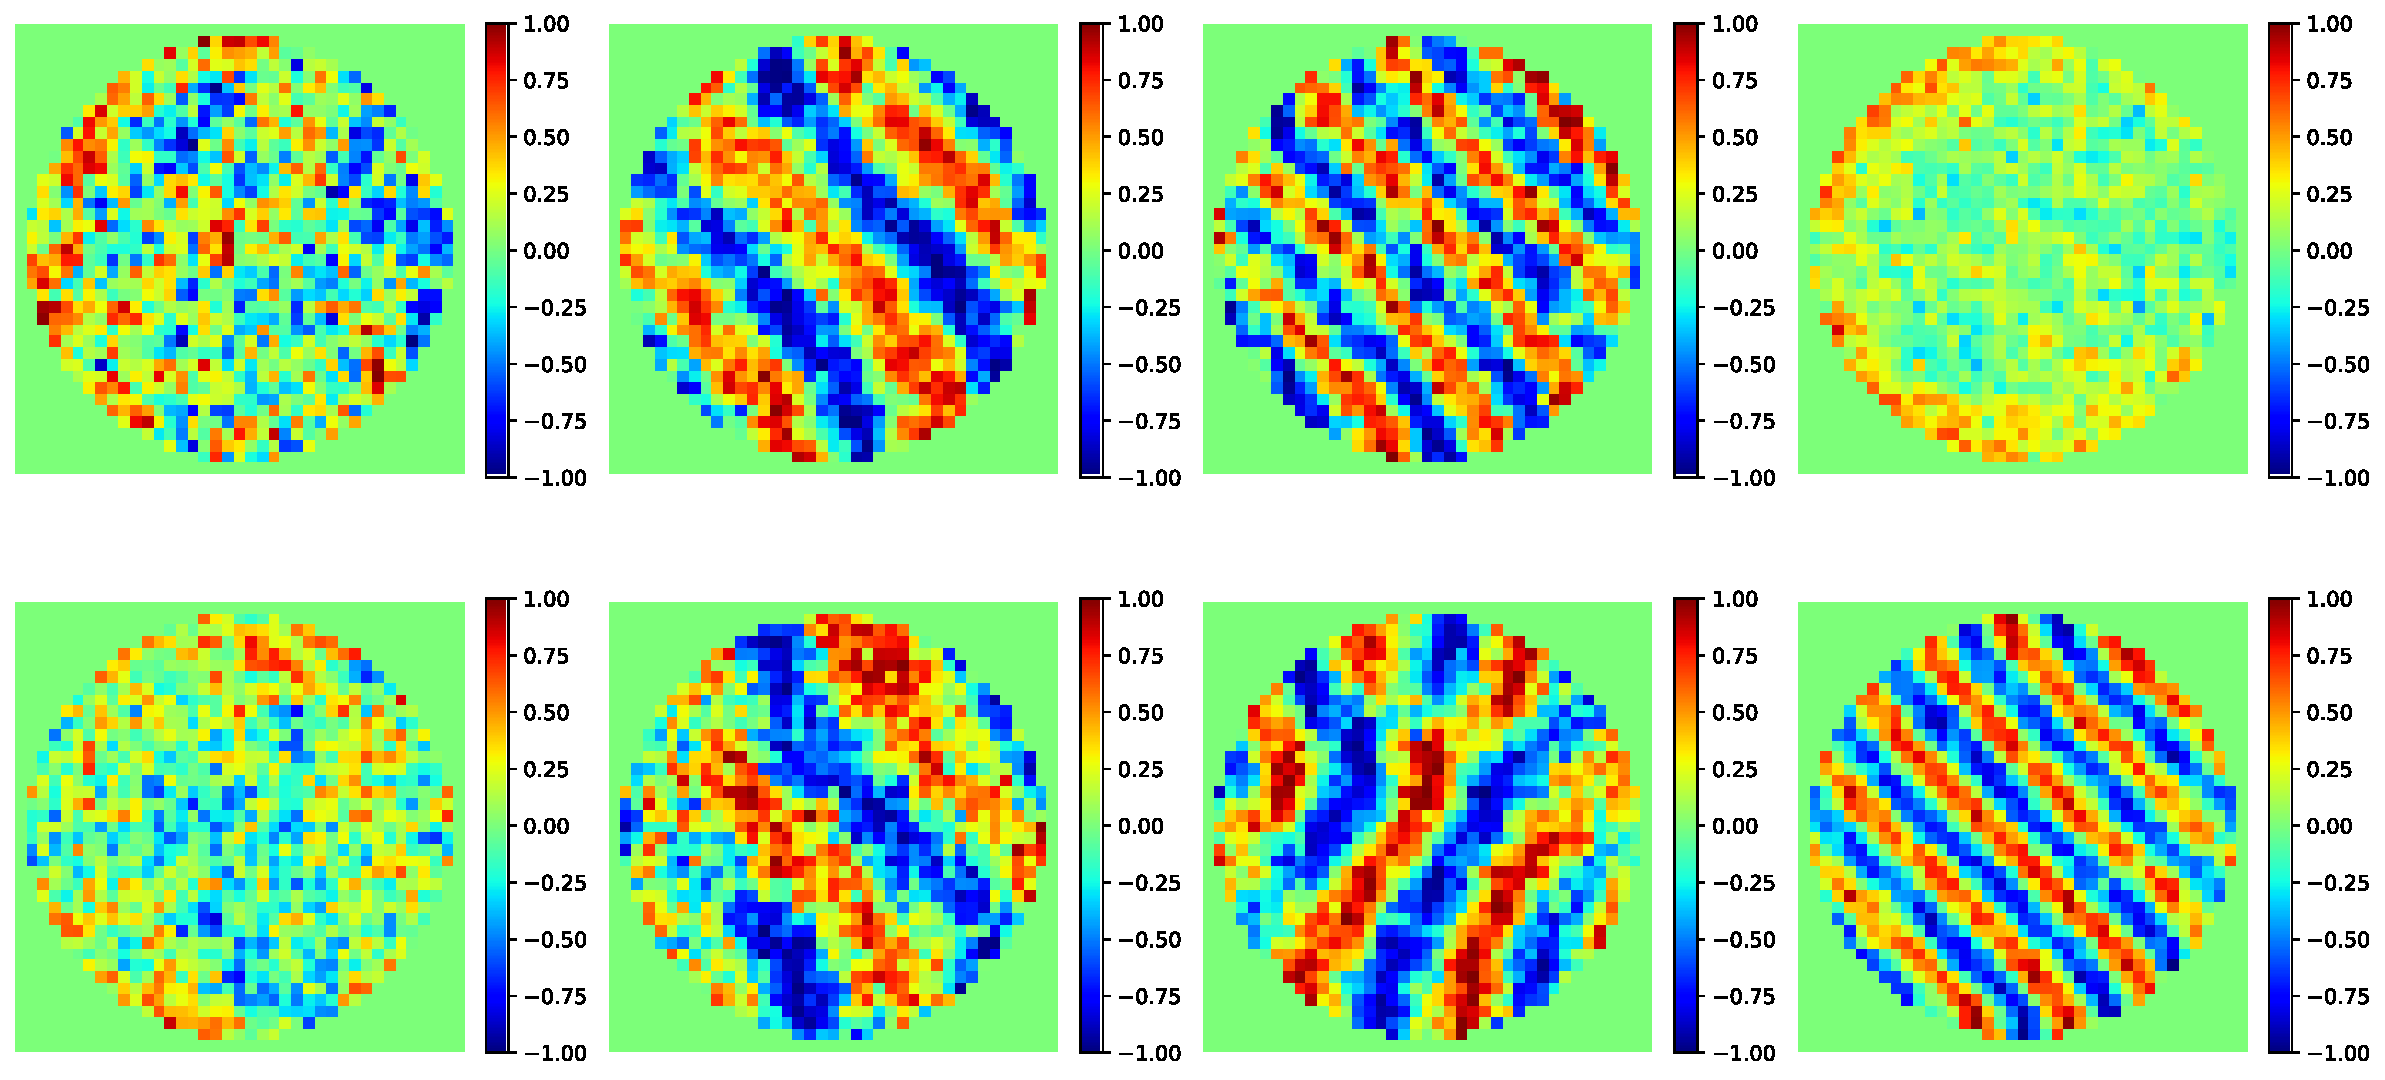
\includegraphics[width=0.85\linewidth]{Figures/imagenes_grid.pdf}
    \caption{Representative examples of magnetic domain configurations from the KDM DATABASE SPINERS dataset. Each image shows a $39 \times 39$ pixel nanodisk spin texture, illustrating the variety of domain patterns (vortices, helical structures, and labyrinthine domains) generated under different combinations of temperature and KDM parameters.}
    \label{fig:kdm_dataset}
\end{figure}

\begin{figure}[H]
    \centering
    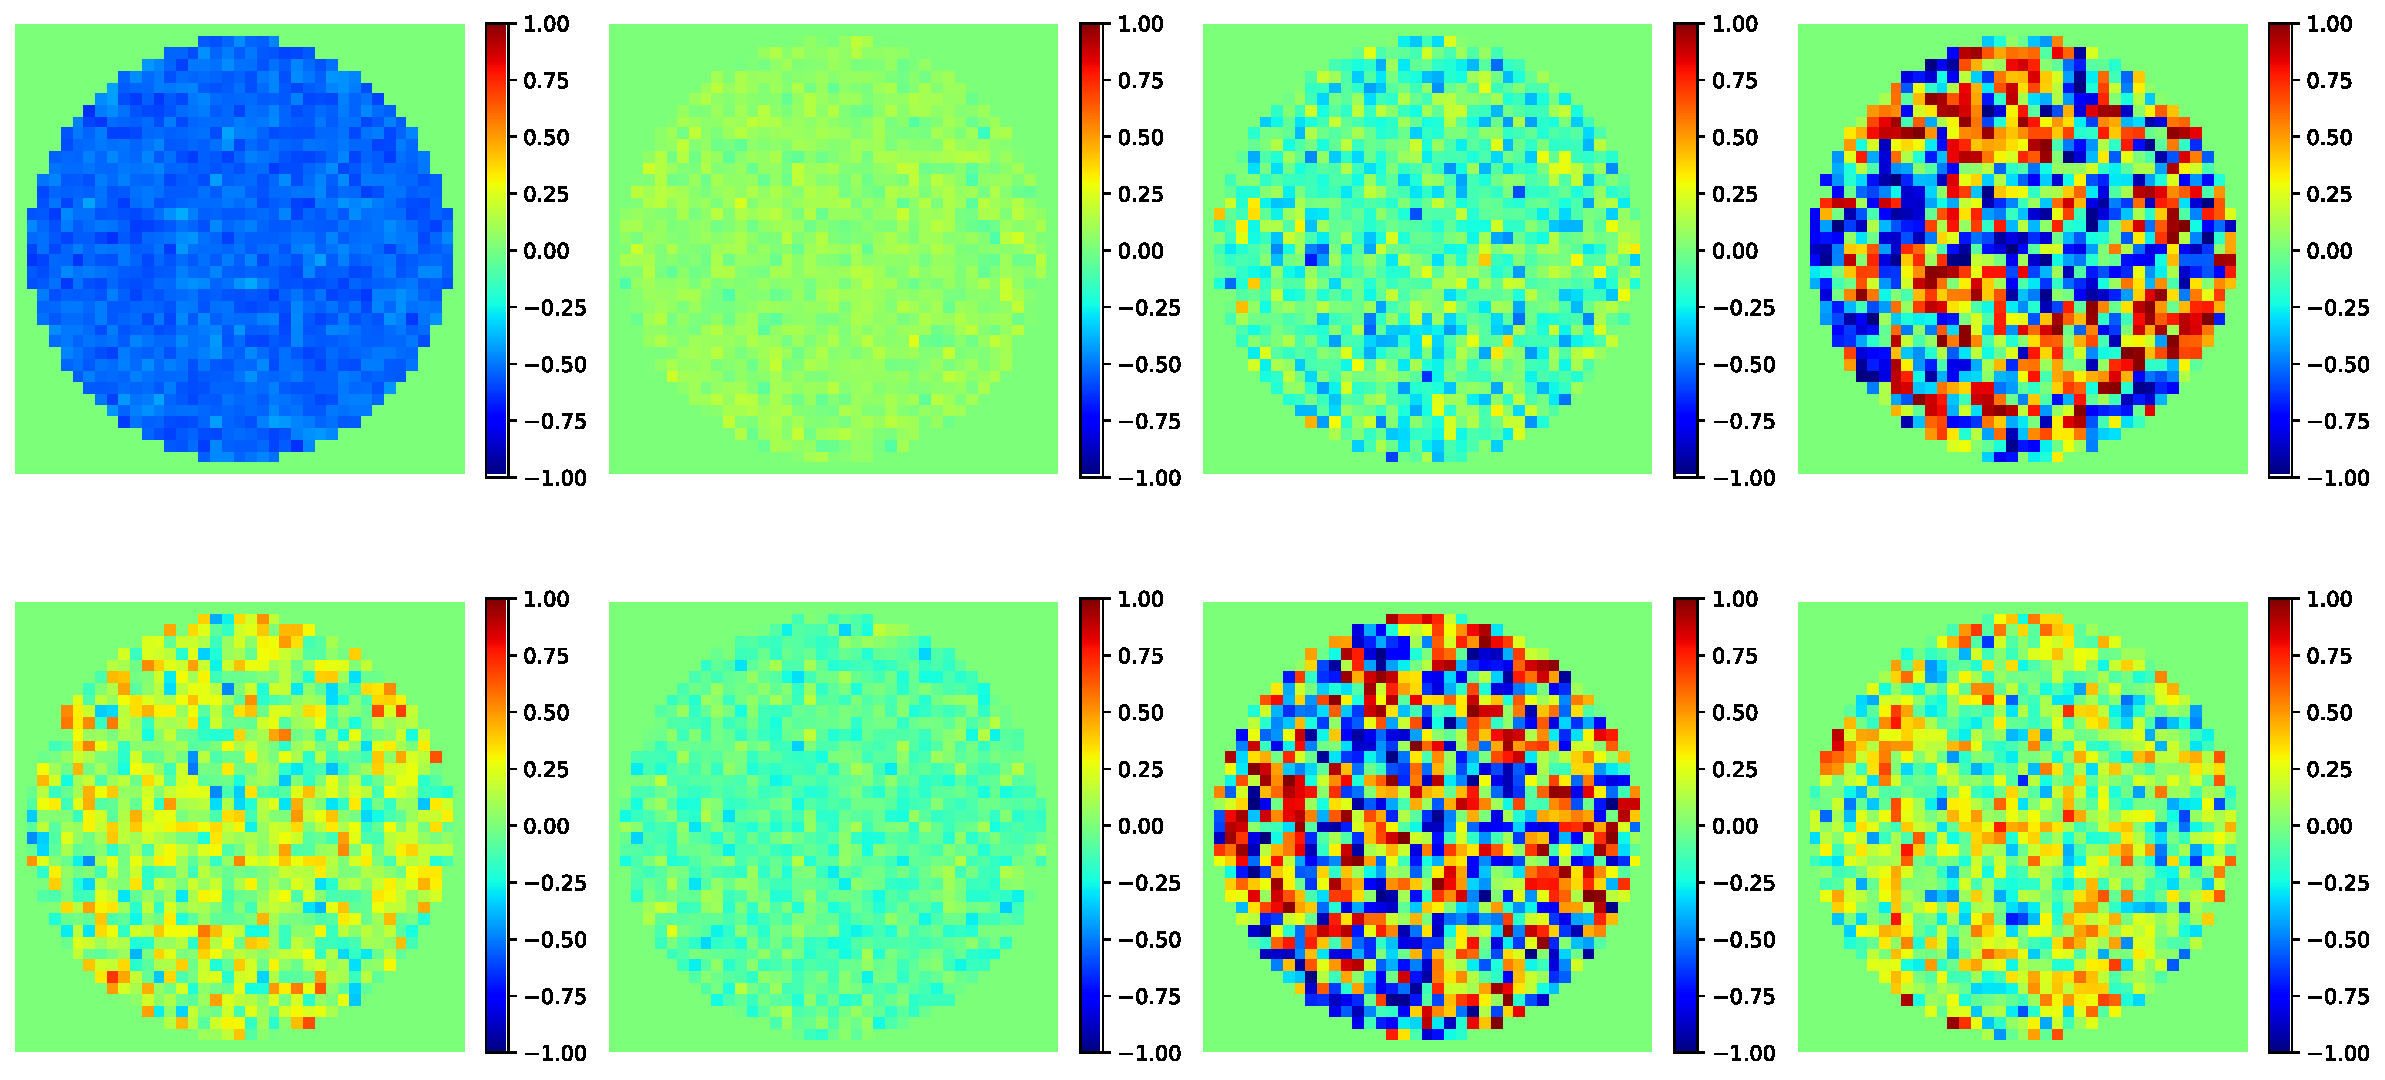
\includegraphics[width=0.85\linewidth]{Figures/imagenes_grid2.pdf}
    \caption{Representative examples of magnetic domain configurations from the MATERIAL SPINNERS DATA dataset. These samples demonstrate spin textures generated under variations in exchange interaction parameters (Jex2) and temperature, exhibiting distinct magnetic morphologies and domain structures.}
    \label{fig:spinner_dataset}
\end{figure}

The distribution of each parameter present in the datasets is shown in Figures~\ref{fig:distribution_kdm} and~\ref{fig:distribution_jex2}. Parameters with nearly uniform distributions across ranges (e.g., \texttt{Kan1}, \texttt{Hex}) indicate that they were sampled broadly, while others with sharp peaks or narrow ranges (e.g., \texttt{rd}, \texttt{kd}) reflect fixed or constrained simulation settings.

\begin{figure}[H]
    \centering
    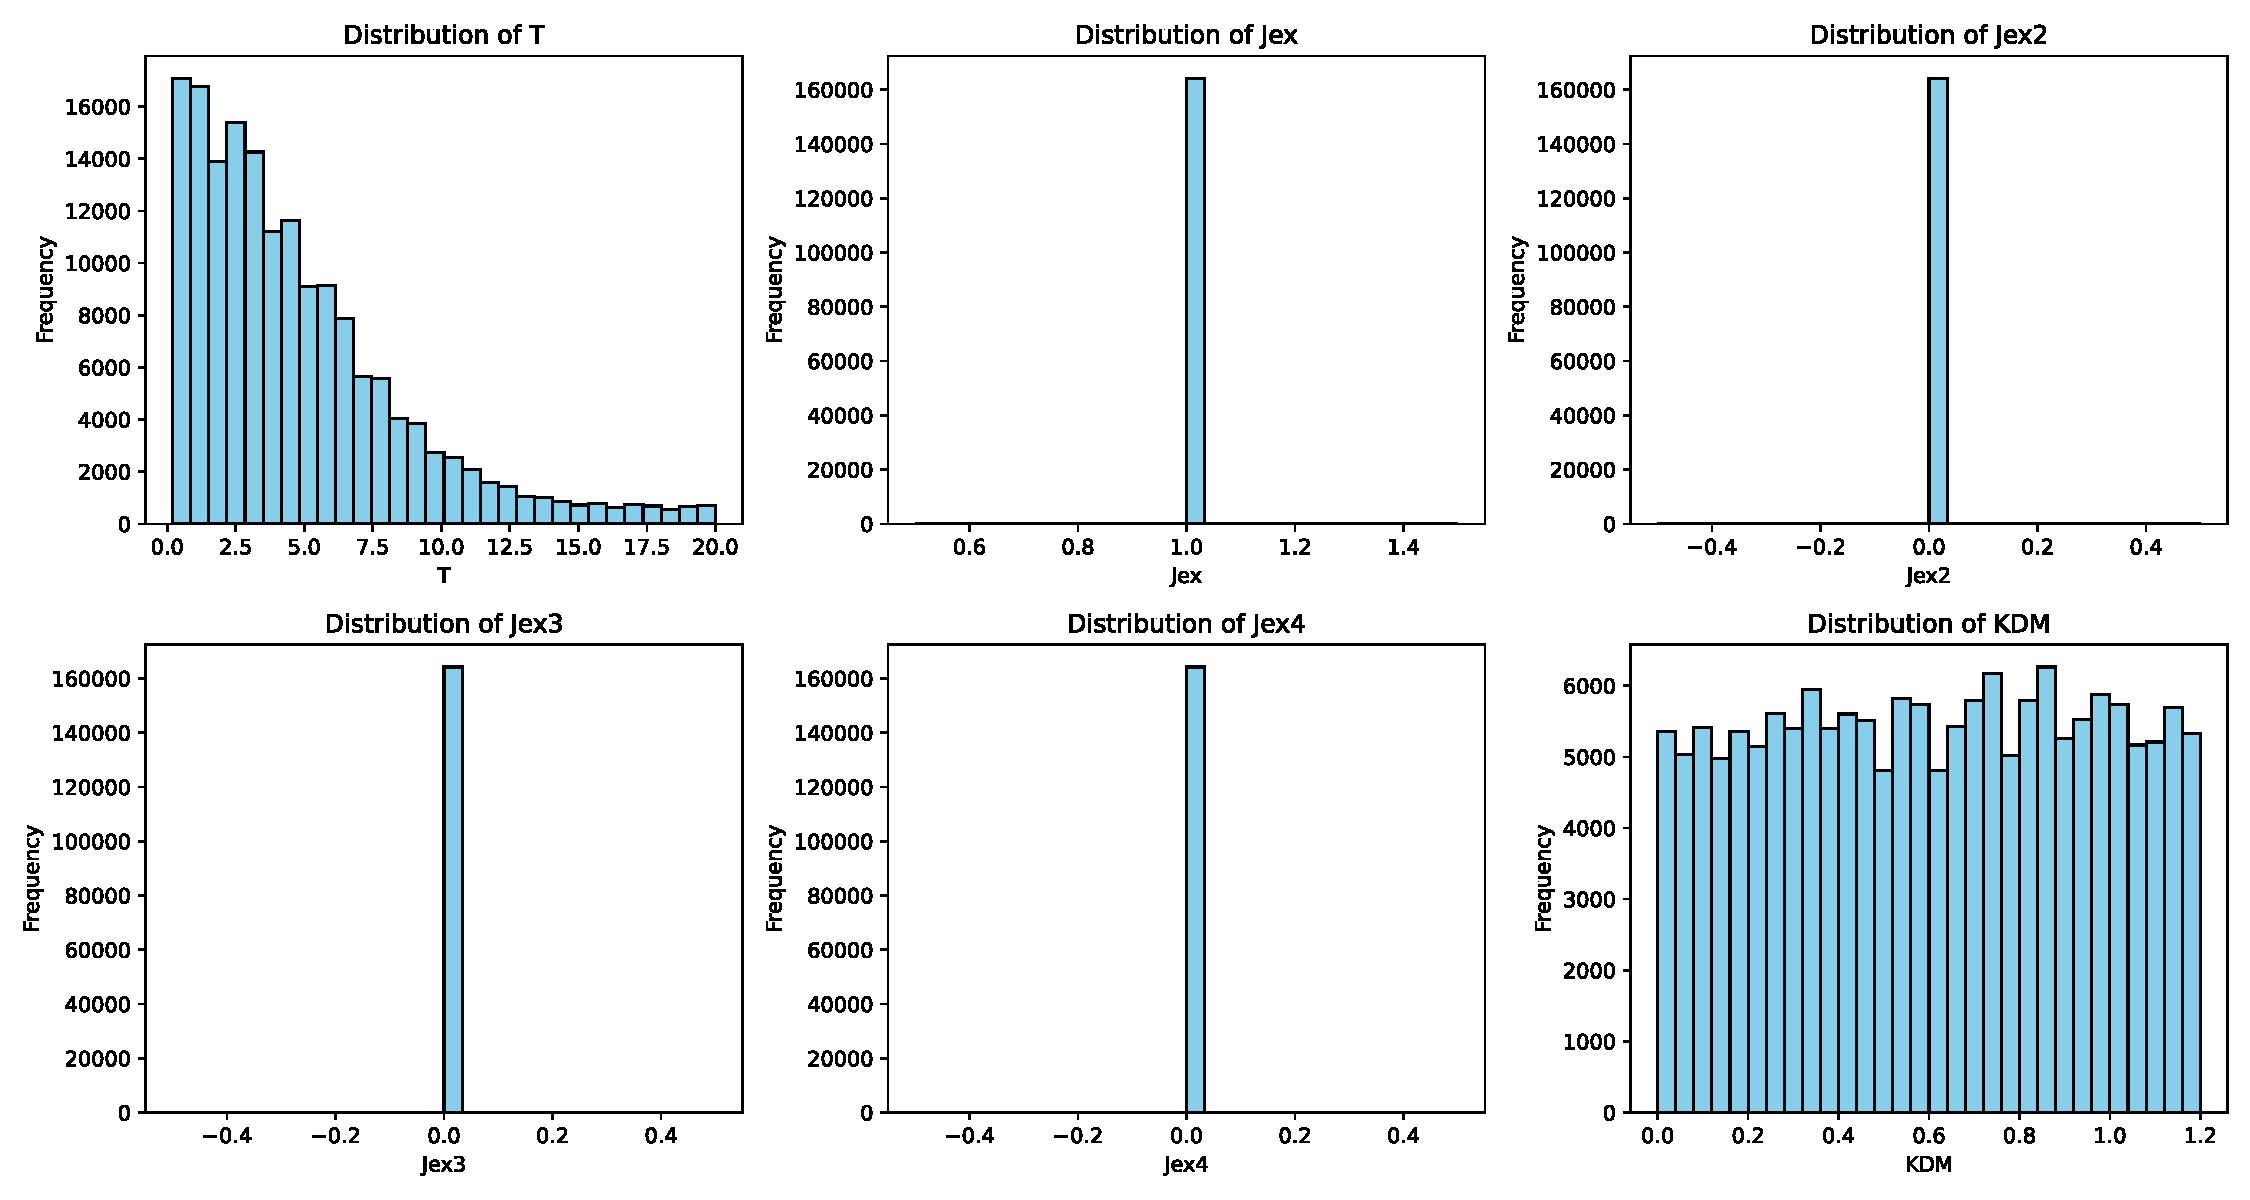
\includegraphics[width=0.85\linewidth]{Figures/distribuciones_parametrosKDM.pdf}
    \caption{Parameter distribution across the full KDM DATABASE SPINERS dataset. Histograms show the frequency distribution of each physical variable, revealing which parameters were varied during simulation (uniform or multimodal distributions) and which were held constant (sharp peaks).}
    \label{fig:distribution_kdm}
\end{figure}

\begin{figure}[H]
    \centering
    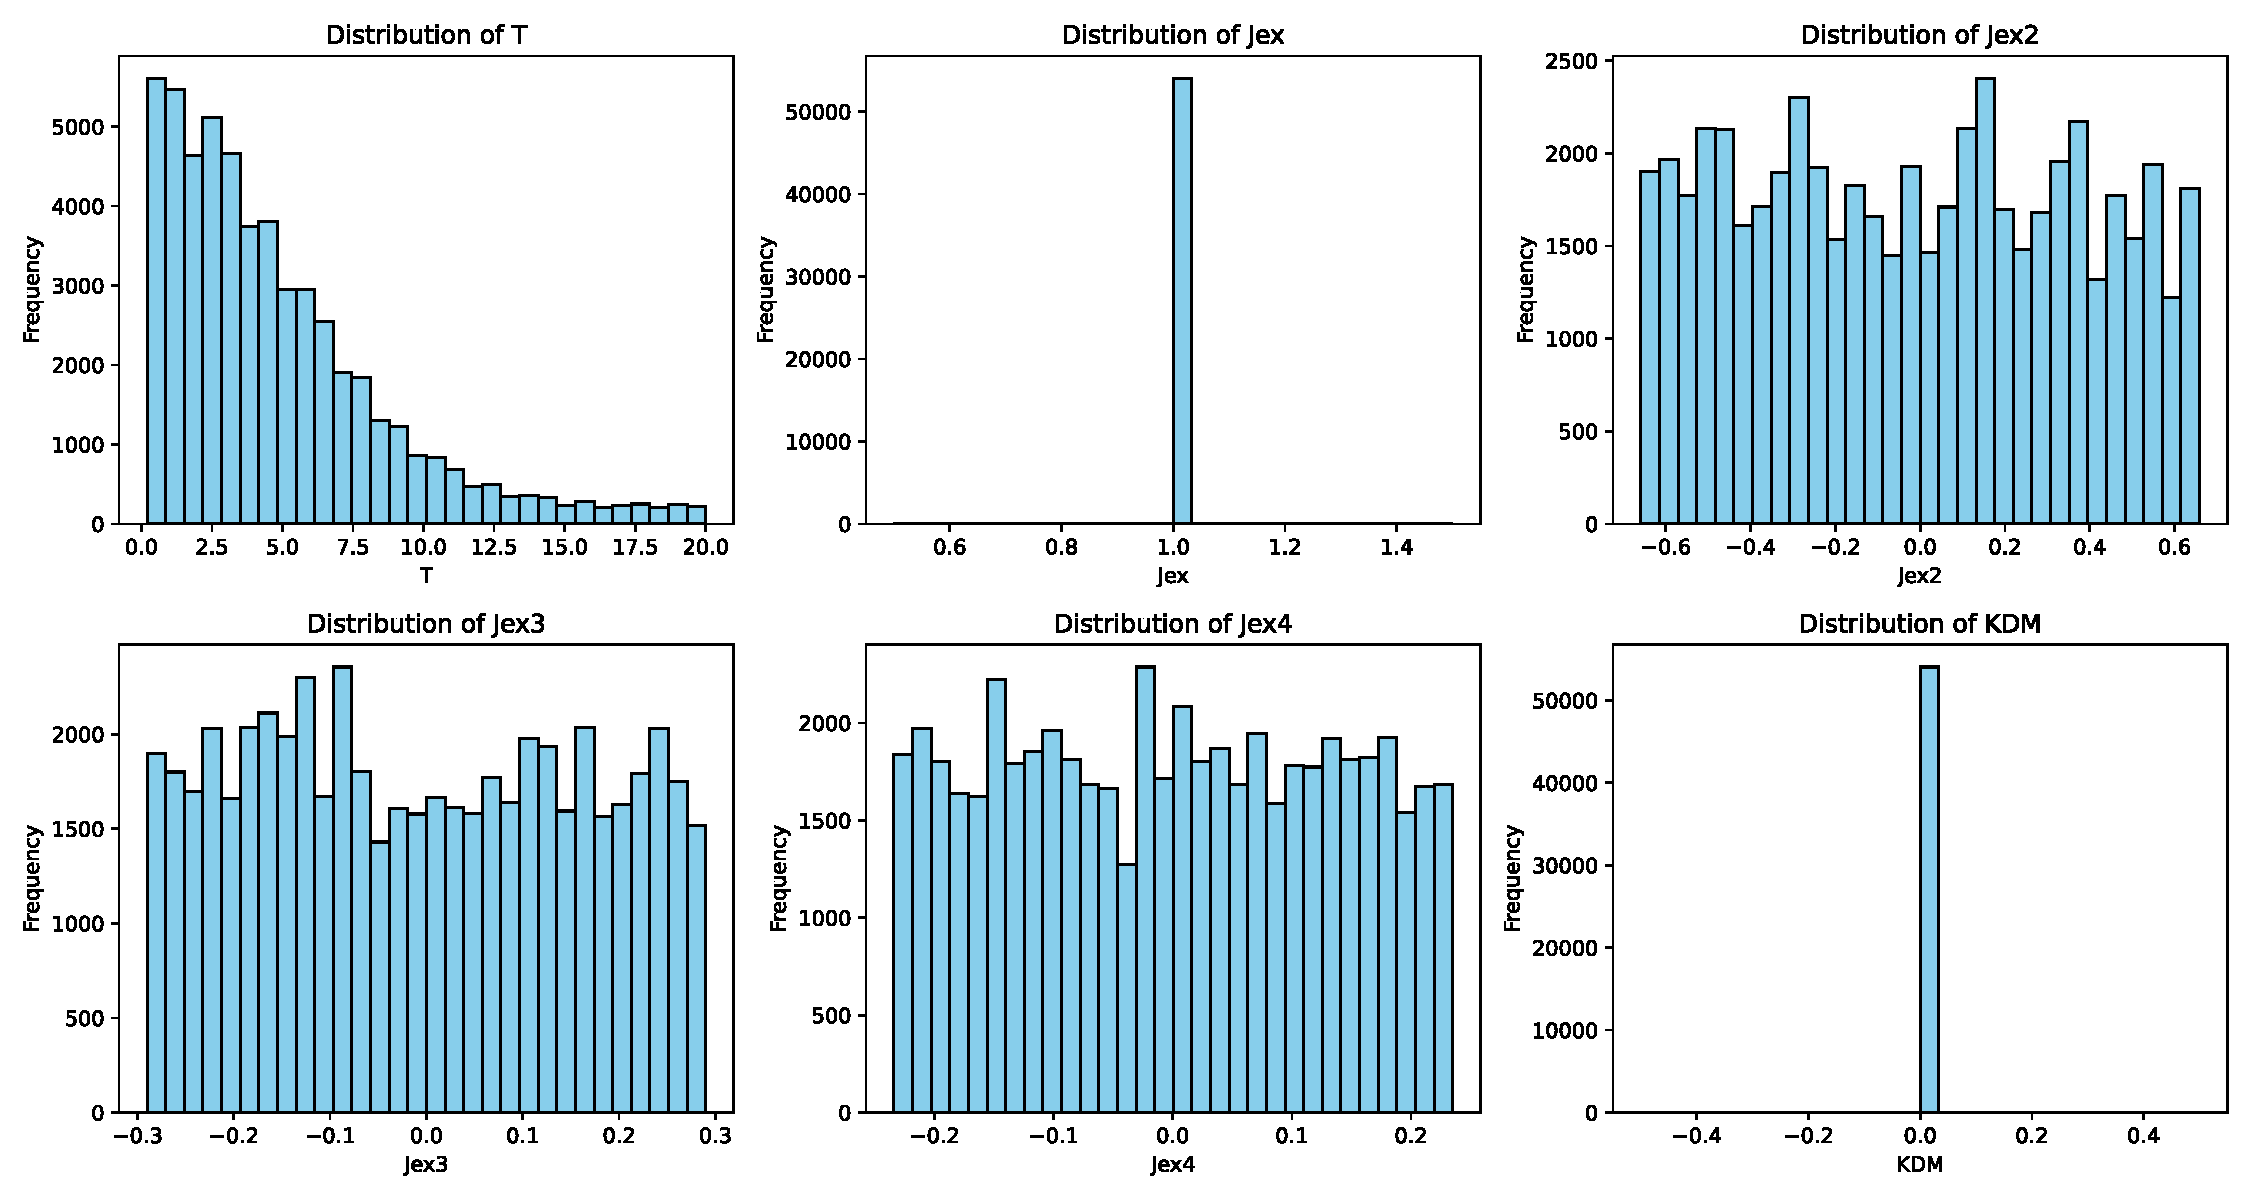
\includegraphics[width=0.85\linewidth]{Figures/distribuciones_parametrosTJex2.pdf}
    \caption{Parameter distribution across the full MATERIAL SPINNERS DATA dataset. The distributions highlight the exploration of exchange interaction parameter space (Jex2) along with temperature variations, showing the coverage of the Hamiltonian parameter space in this complementary dataset.}
    \label{fig:distribution_jex2}
\end{figure}

\subsection{Proof of Concept: Conditional Variational Autoencoder with Physics-Guided Conditioning}

To address the first research objective—mitigating the effect of magnetic state degeneracy in configuration estimation tasks—we developed and evaluated a proof-of-concept implementation of a Conditional Variational Autoencoder (cVAE) with physics-guided parameter conditioning. This initial exploration focuses on establishing the baseline generative capabilities of the architecture before incorporating explicit physical constraints.

The proposed architecture, illustrated in Figure~\ref{fig:cvae_architecture}, implements a learned conditional prior $p_\theta(z|c)$ that depends on physical parameters $c$ (temperature $T$ and the derived KDM parameter combining anisotropy and Dzyaloshinskii–Moriya interactions), rather than imposing a fixed standard normal prior as in classical VAEs. This design choice aims to structure the latent space according to the underlying Hamiltonian parameter space, thereby reducing ambiguities arising from parameter degeneracy.

\begin{figure}[H]
    \centering
    \includegraphics[width=0.85\textwidth]{Figures/cVae.png}
    \caption{Conditional VAE architecture with physics-guided parameter conditioning. The encoder $Q_\phi$ maps input magnetic configurations $x$ to a latent distribution $q_\phi(z|x,c)$ conditioned on physical parameters $c$. The prior network $P_\psi$ learns a parameter-dependent latent prior $p_\psi(z|c)$, while the decoder $G_\theta$ reconstructs magnetic configurations from sampled latent codes and conditions.}
    \label{fig:cvae_architecture}
\end{figure}

\subsubsection{Architecture Design}

The model comprises three main components: an encoder $Q_\phi$, a decoder $G_\theta$, and a prior network $P_\psi$, all conditioned on the physical parameter vector $c \in \mathbb{R}^2$ (temperature and KDM).

\paragraph{Encoder Architecture.}
The encoder $Q_\phi$ projects the input image $x \in \mathbb{R}^{39 \times 39}$ to a low-dimensional latent space $z \in \mathbb{R}^d$, conditioned by $c$. The architecture follows a hybrid design:

\begin{itemize}
    \item \textbf{Visual Processing}: The image passes through a series of convolutional blocks (Conv2D) responsible for spatial feature extraction. Each block reduces spatial dimensionality while increasing the depth of feature maps.
    \item \textbf{Condition Fusion}: The vector $c$ is processed via a linear layer and concatenated with the flattened visual feature vector resulting from the convolutions.
    \item \textbf{Latent Projection}: The fused vector feeds two separate linear layers that predict the mean $\mu_{\text{enc}}$ and the logarithm of the variance $\log(\sigma^2_{\text{enc}})$ of the approximate posterior distribution $q_\phi(z|x,c)$.
\end{itemize}

During training, the reparameterization trick is used to sample $z$:
\begin{equation}
z = \mu_{\text{enc}} + \sigma_{\text{enc}} \cdot \varepsilon, \quad \varepsilon \sim \mathcal{N}(0, I).
\end{equation}

\paragraph{Decoder Architecture.}
The decoder $G_\theta$ acts as the system generator, performing the inverse operation to the encoder:

\begin{itemize}
    \item \textbf{Input}: Receives the sampled latent vector $z$ concatenated with the condition vector $c$, ensuring that generation respects physical constraints at each step.
    \item \textbf{Upsampling}: The fused input is projected via a dense layer and reshaped to form an initial spatial tensor.
    \item \textbf{Reconstruction}: A series of transposed convolution layers (ConvTranspose2D) progressively increase the spatial dimension until recovering the original size of $39 \times 39$ pixels.
    \item \textbf{Output Activation}: The final layer uses a sigmoid activation function to guarantee that output pixel values $\hat{x}$ are bounded in the range $[0, 1]$, consistent with the input data normalization.
\end{itemize}

\paragraph{Prior Network.}
Unlike standard VAEs that impose a fixed $p(z) = \mathcal{N}(0, I)$, the conditional prior $p_\psi(z|c)$ introduces a physics-shaped structure into the latent space:
\begin{equation}
p_\psi(z|c) = \mathcal{N}\left(\mu_\psi(c), \Sigma_\psi(c)\right),
\end{equation}
where $\mu_\psi$ and $\Sigma_\psi$ are neural networks that learn a latent distribution consistent with the Hamiltonian's parameter space. This formulation prevents the model from collapsing physically distinct regimes into overlapping latent regions, reducing degeneracy by enforcing that different parameter vectors induce distinct latent priors.

\subsubsection{Loss Function Implementation}

For this proof of concept, we implemented a simplified loss function without explicit physical constraints, focusing on reconstruction fidelity and latent space regularization. The total loss $\mathcal{L}$ minimized during training is:
\begin{equation}
\mathcal{L} = \mathcal{L}_{\text{recon}}(x, \hat{x}) + \beta \cdot D_{\text{KL}}\left(q_\phi(z|x,c) \,\|\, p_\psi(z|c)\right),
\end{equation}
where:

\paragraph{Reconstruction Loss.}
Mean Squared Error (MSE) measures pixel-to-pixel fidelity between the original and generated image:
\begin{equation}
\mathcal{L}_{\text{recon}} = \frac{1}{N} \sum_{i=1}^{N} \|x_i - \hat{x}_i\|^2.
\end{equation}

\paragraph{Conditional KL Divergence.}
The KL divergence regularizes the posterior distribution by enforcing proximity to a parameter-dependent latent prior:
\begin{equation}
\mathcal{L}_{\text{KL}} = D_{\text{KL}}\left(q_\phi(z|x,c) \,\|\, p_\psi(z|c)\right).
\end{equation}

Unlike classical VAEs, the conditional prior $p_\psi(z|c)$ introduces a physics-shaped structure into the latent space. Since both the encoder posterior $q_\phi(z|x,c) = \mathcal{N}(\mu_1, \sigma_1^2)$ and the prior $p_\psi(z|c) = \mathcal{N}(\mu_2, \sigma_2^2)$ are Gaussian, the KL divergence admits an analytical solution:
\begin{equation}
D_{\text{KL}} = \frac{1}{2} \sum_{j=1}^{d} \left[ \log\frac{\sigma_{2,j}^2}{\sigma_{1,j}^2} + \frac{\sigma_{1,j}^2 + (\mu_{1,j} - \mu_{2,j})^2}{\sigma_{2,j}^2} - 1 \right],
\end{equation}
where $(\mu_1, \sigma_1)$ come from the encoder $q(z|x,c)$, $(\mu_2, \sigma_2)$ come from the prior network $p(z|c)$, and $d$ is the dimension of the latent space. The hyperparameter $\beta$ (Beta-VAE) controls the regularization weight, allowing a balance between reconstruction quality and latent space structure.

\subsubsection{Experimental Setup and Results}

For this proof of concept, we trained the cVAE exclusively on the KDM DATABASE SPINERS dataset, focusing on two physical parameters: temperature $T$ and the derived KDM parameter. The model was trained without explicit physics-based regularization ($\mathcal{L}_{\text{phys}} = 0$) to establish baseline generative performance and evaluate the intrinsic capability of the conditional prior to structure the latent space according to physical parameters.

\paragraph{Latent Space Organization.}
To assess whether the learned latent space encodes physically meaningful structure, we applied UMAP (Uniform Manifold Approximation and Projection) dimensionality reduction to the latent representations $z$ of the test set. Figures~\ref{fig:umap_tkdm} and~\ref{fig:umap_images} visualize the resulting two-dimensional embeddings, colored by temperature and KDM values, and overlaid with representative magnetic domain configurations, respectively.

\begin{figure}[H]
    \centering
    \includegraphics[width=0.95\textwidth]{Figures/UmapDirectTKDM.png}
    \caption{UMAP projection of the latent space learned by the conditional VAE, colored by physical parameters. Left: temperature $T$; Right: KDM parameter. The visualization reveals that the latent space exhibits smooth gradients corresponding to variations in physical parameters, indicating that the conditional prior successfully structures the latent manifold according to the underlying Hamiltonian parameter space.}
    \label{fig:umap_tkdm}
\end{figure}

\begin{figure}[H]
    \centering
    \includegraphics[width=0.85\textwidth]{Figures/UmapDirect.png}
    \caption{UMAP projection of the latent space with representative magnetic domain configurations overlaid on their corresponding latent positions. The spatial organization of domain morphologies (vortices, helical structures, labyrinthine patterns) suggests that the model has learned to cluster physically similar configurations in nearby latent regions, even without explicit physics-based constraints.}
    \label{fig:umap_images}
\end{figure}

The UMAP projections demonstrate that the conditional prior successfully induces a physically meaningful latent geometry. Despite the absence of explicit physical regularization, the latent space exhibits smooth gradients aligned with variations in temperature and KDM, and morphologically similar magnetic configurations cluster together. This result suggests that the parameter-conditioned prior $p_\psi(z|c)$ effectively reduces latent degeneracy by enforcing that distinct physical conditions correspond to distinct latent distributions.

\paragraph{Generative Quality.}
To evaluate the reconstruction and generative fidelity of the model, we compared ground-truth magnetic configurations from the test set with their reconstructions produced by the cVAE. Figure~\ref{fig:generation} presents a qualitative comparison across a range of physical conditions.

\begin{figure}[H]
    \centering
    \includegraphics[width=0.95\textwidth]{Figures/Generation.png}
    \caption{Comparison between ground-truth magnetic domain configurations (top rows) and their reconstructions generated by the conditional VAE (bottom rows). The model successfully captures the main topological features of the magnetic textures—including vortex cores, domain wall structures, and edge effects—demonstrating that the architecture achieves high-fidelity reconstruction even without explicit physics-based constraints. Minor discrepancies in fine-scale details suggest opportunities for further improvement through physics-informed regularization.}
    \label{fig:generation}
\end{figure}

The reconstructions exhibit high qualitative fidelity, capturing the primary topological features of magnetic domain structures, including vortex cores, domain walls, and edge-induced patterns. Minor deviations in fine-scale details are observed, particularly in regions with complex spin textures, indicating that while the baseline cVAE achieves strong generative performance, the incorporation of explicit physics-based constraints (such as energy penalties or LLG residuals) may further improve physical consistency and reduce reconstruction artifacts.

\paragraph{Discussion.}
This proof-of-concept evaluation demonstrates that the conditional VAE with learned physics-guided priors provides a promising foundation for addressing magnetic state degeneracy. The key findings are:

\begin{itemize}
    \item \textbf{Latent Space Structure}: The parameter-conditioned prior $p_\psi(z|c)$ successfully organizes the latent space according to physical parameters, as evidenced by smooth UMAP gradients and physically coherent clustering, even in the absence of explicit energy or dynamics constraints.
    \item \textbf{Reconstruction Fidelity}: The model achieves high-quality reconstructions of complex magnetic textures, capturing essential topological features while maintaining pixel-level accuracy suitable for downstream tasks.
    \item \textbf{Baseline for Physics-Informed Extensions}: The results establish a baseline against which future enhancements—including Hamiltonian energy penalties, cycle-consistency constraints, and transfer learning to experimental data—can be systematically evaluated.
\end{itemize}

\paragraph{Identified Limitations and Future Refinements.}
Despite these encouraging results, this proof-of-concept implementation reveals critical methodological challenges that must be addressed before deployment:

\begin{itemize}
    \item \textbf{Hyperparameter Optimization}: The current architecture was trained with manually selected hyperparameters. To fully exploit the model's capacity, a systematic Bayesian optimization procedure (e.g., using Optuna~\cite{Optuna2022}) must be conducted to identify optimal values for $\beta$, latent dimensionality $d$, learning rates, and network depth. The baseline performance reported here likely underestimates the architecture's true potential.

    \item \textbf{Pixel-Level Metrics and Geometric Invariance}: A fundamental limitation emerged during evaluation: magnetic domain configurations are inherently invariant to spatial transformations (rotations, translations, and reflections). Two configurations that differ only by a rigid transformation are \textit{physically equivalent}, yet pixel-wise metrics such as MSE assign them high dissimilarity. This misalignment between the evaluation metric and the physical equivalence relation leads to systematically underestimated generative quality. Figure~\ref{fig:generation} qualitatively demonstrates that the model can produce physically coherent states, but quantitative assessment via MSE penalizes geometrically transformed yet physically valid outputs. Alternative evaluation strategies must be explored, including:
    \begin{itemize}
        \item \textit{Rotation- and translation-invariant metrics} based on topological descriptors (e.g., skyrmion number, vorticity fields, or Betti numbers).
        \item \textit{Energy-based metrics} that assess the physical consistency of generated states through micromagnetic energy functionals rather than pixel-level comparisons.
        \item \textit{Structural similarity measures} (e.g., Fréchet Inception Distance adapted to magnetic textures) that capture perceptual and physical similarity beyond pixel alignment.
    \end{itemize}
\end{itemize}

These findings validate the feasibility of the proposed architecture and motivate the subsequent integration of physics-informed regularization to further reduce degeneracy, improve generalization to unseen parameter regimes, and ensure strict adherence to micromagnetic principles. Moreover, they highlight the necessity of developing evaluation protocols that respect the geometric symmetries inherent to magnetic domain structures.


\subsection{Proof of Concept: Inverse Problem for Parameter Estimation via Transfer Learning}

Having established a baseline for the generative modeling of magnetic domain states through the conditional VAE, we now address the \textit{inverse problem}: the task of estimating underlying physical parameters from observed magnetic configurations. This complementary direction is critical for the long-term objective of integrating forward (state generation) and inverse (parameter inference) workflows into a unified physics-informed framework. In this proof-of-concept, we explore the feasibility of multivariate regression from spin structure images to physical parameters using convolutional neural networks (CNNs) trained via transfer learning. Additionally, we introduce a novel passive interpretability method—\textit{Regression Activation Maps (RAMs)}—to identify which spatial regions of the input contribute most to accurate predictions.

\subsubsection{Problem Formulation and Architecture Design}

The inverse problem is formulated as a multivariate regression task, where the model $f_\theta: \mathbb{R}^{H \times W} \to \mathbb{R}^p$ maps an input image representing the material's spin structure to a vector of $p$ physical parameters. For the KDM DATABASE SPINERS, the target variables are temperature $T$ and the Dzyaloshinskii–Moriya interaction magnitude $KDM$. For the MATERIAL SPINNERS DATA, we predict $T$, $J_{ex2}$, $J_{ex3}$, and $J_{ex4}$.

Due to computational constraints, a representative subset of 50,000 images was selected from the full dataset, preserving the original distributions of physical variables. The approach is based on \textit{transfer learning}, leveraging pretrained image encoders from state-of-the-art computer vision architectures to extract high-level representations from spin configurations before performing regression. Pretrained weights from ImageNet are employed, allowing the model to benefit from learned visual features and accelerate convergence. The final classification layers of the original architectures are replaced with regression-specific dense layers, enabling multivariate continuous output.

\begin{figure}[H]
\centering
\includegraphics[width=0.75\linewidth]{Figures/Esquema.png}
\caption{Schematic representation of the transfer learning pipeline for inverse parameter estimation. A pretrained CNN encoder extracts high-dimensional features from the magnetic domain image, which are then mapped to physical parameters via regression-specific layers.}
\label{fig:inverse_schema}
\end{figure}

The architectures implemented, all available in TensorFlow, are summarized in Table~\ref{tab:architectures_inverse}.

\begin{table}[H]
\centering
\footnotesize
\caption{Deep learning architectures evaluated for inverse parameter estimation.}
\label{tab:architectures_inverse}
\begin{tabular}{ll}
\toprule
\textbf{Model} & \textbf{Description / Notes} \\
\midrule
DenseNet121    & Dense Convolutional Network, 121 layers \\
ResNet50       & Residual Network, 50 layers \\
Inception      & Inception v3 architecture \\
EfficientNetB0 & EfficientNet baseline model (lightweight) \\
EfficientNetB2 & Scaled EfficientNet variant (deeper than B0) \\
\bottomrule
\end{tabular}
\end{table}

\paragraph{Training Details.}
All convolutional models were trained using the Adam optimizer with mean squared error (MSE) as the primary loss function:
\begin{equation}
\mathcal{L}_{\text{MSE}} = \frac{1}{n} \sum_{i=1}^n \left(y_i - \hat{y}_i\right)^2,
\end{equation}
and mean absolute error (MAE) as a complementary evaluation metric:
\begin{equation}
\text{MAE} = \frac{1}{n} \sum_{i=1}^n \left|y_i - \hat{y}_i\right|.
\end{equation}

The dataset was split into 80\% training, 10\% validation, and 10\% testing. Data normalization was performed using MinMaxScaler from scikit-learn. Models were trained for 10 epochs on an A100 GPU (Google Colab). Performance was evaluated using the coefficient of determination ($R^2$) and symmetric mean absolute percentage error (SMAPE):
\begin{equation}
R^2 = 1 - \frac{\sum_{i=1}^{n} (y_i - \hat{y}_i)^2}{\sum_{i=1}^{n} (y_i - \bar{y})^2},
\end{equation}
\begin{equation}
\text{SMAPE} = \frac{100}{n} \sum_{i=1}^n \frac{|y_i - \hat{y}_i|}{(|y_i| + |\hat{y}_i|)/2}.
\end{equation}

\subsubsection{Model Comparison and Selection}

To assess predictive performance across the selected physical parameters, we evaluated five CNN encoder architectures on both datasets. Figures~\ref{fig:comparison_kdm_inverse} and~\ref{fig:comparison_jex2_inverse} summarize the results for the two target variables (KDM and T for the KDM DATABASE; $J_{ex2}$, $J_{ex3}$, $J_{ex4}$, and T for the MATERIAL SPINNERS DATA).

\begin{figure}[H]
    \centering
    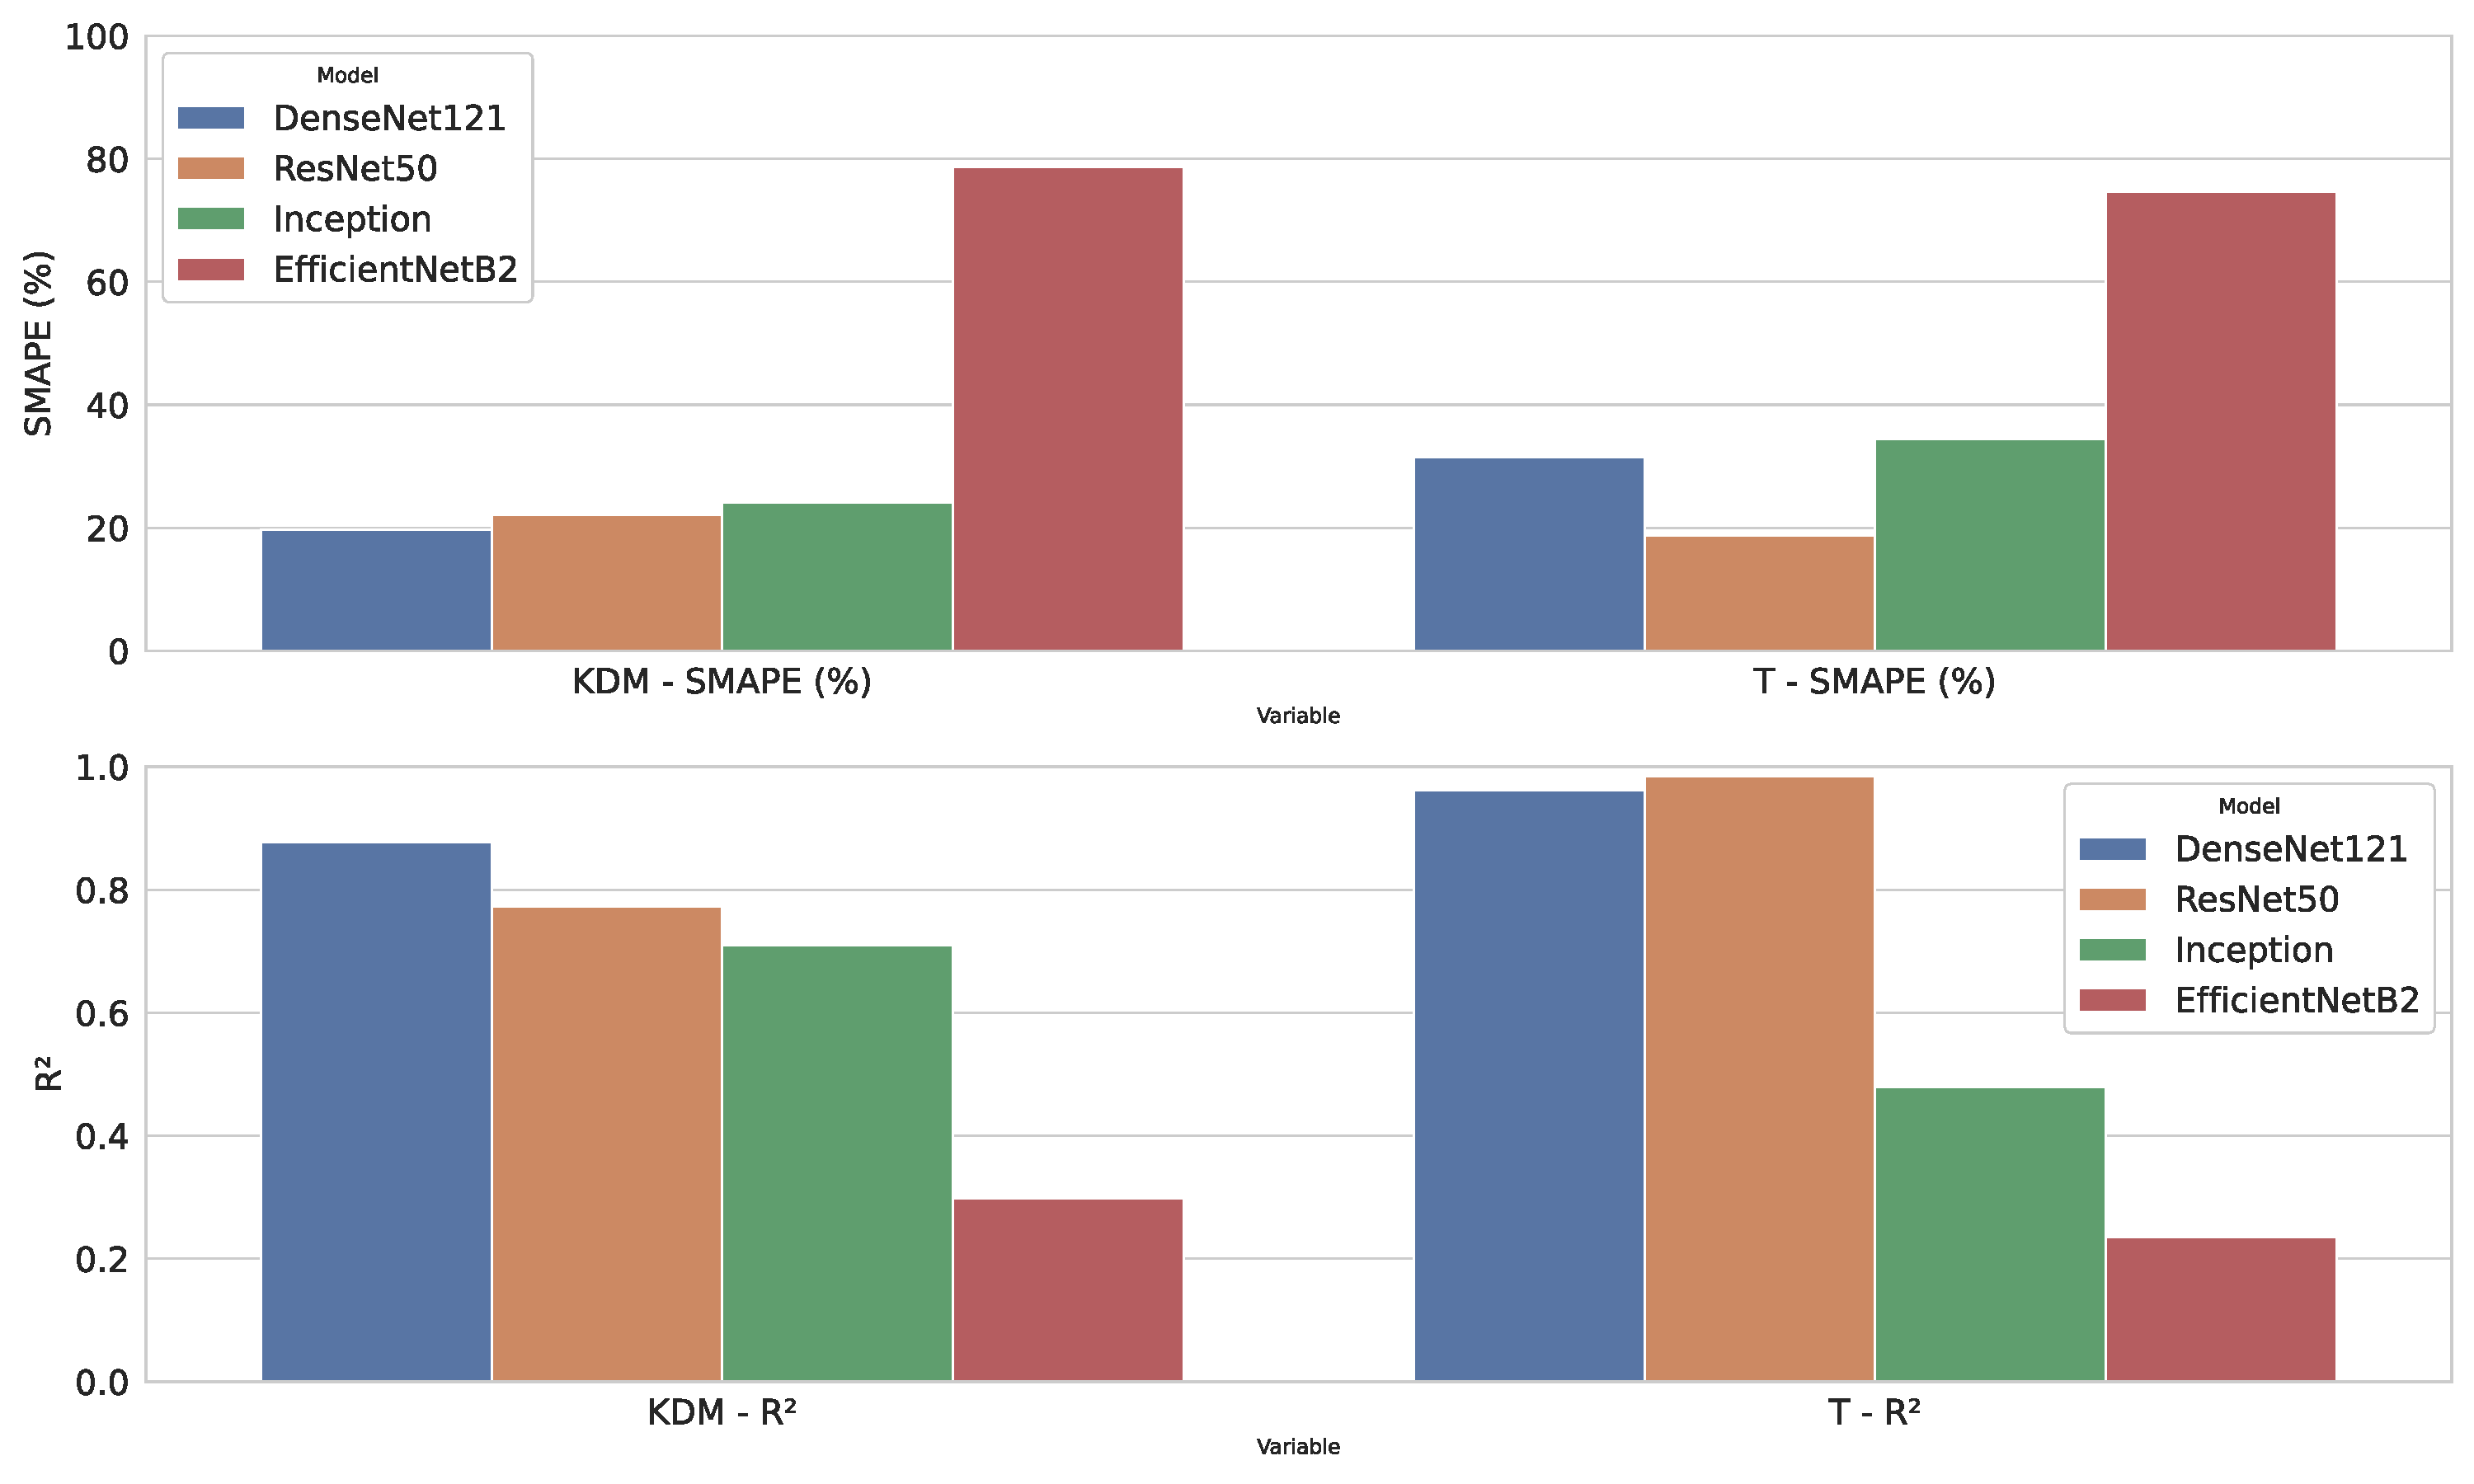
\includegraphics[width=0.95\linewidth]{Figures/comparacion_modelos_separados_KDM.pdf}
    \caption{Model comparison for the KDM DATABASE SPINERS: $R^2$ and SMAPE across five CNN architectures for temperature (T) and Dzyaloshinskii–Moriya interaction (KDM) estimation. DenseNet121 achieves the best balance, particularly for KDM.}
    \label{fig:comparison_kdm_inverse}
\end{figure}

\begin{figure}[H]
    \centering
    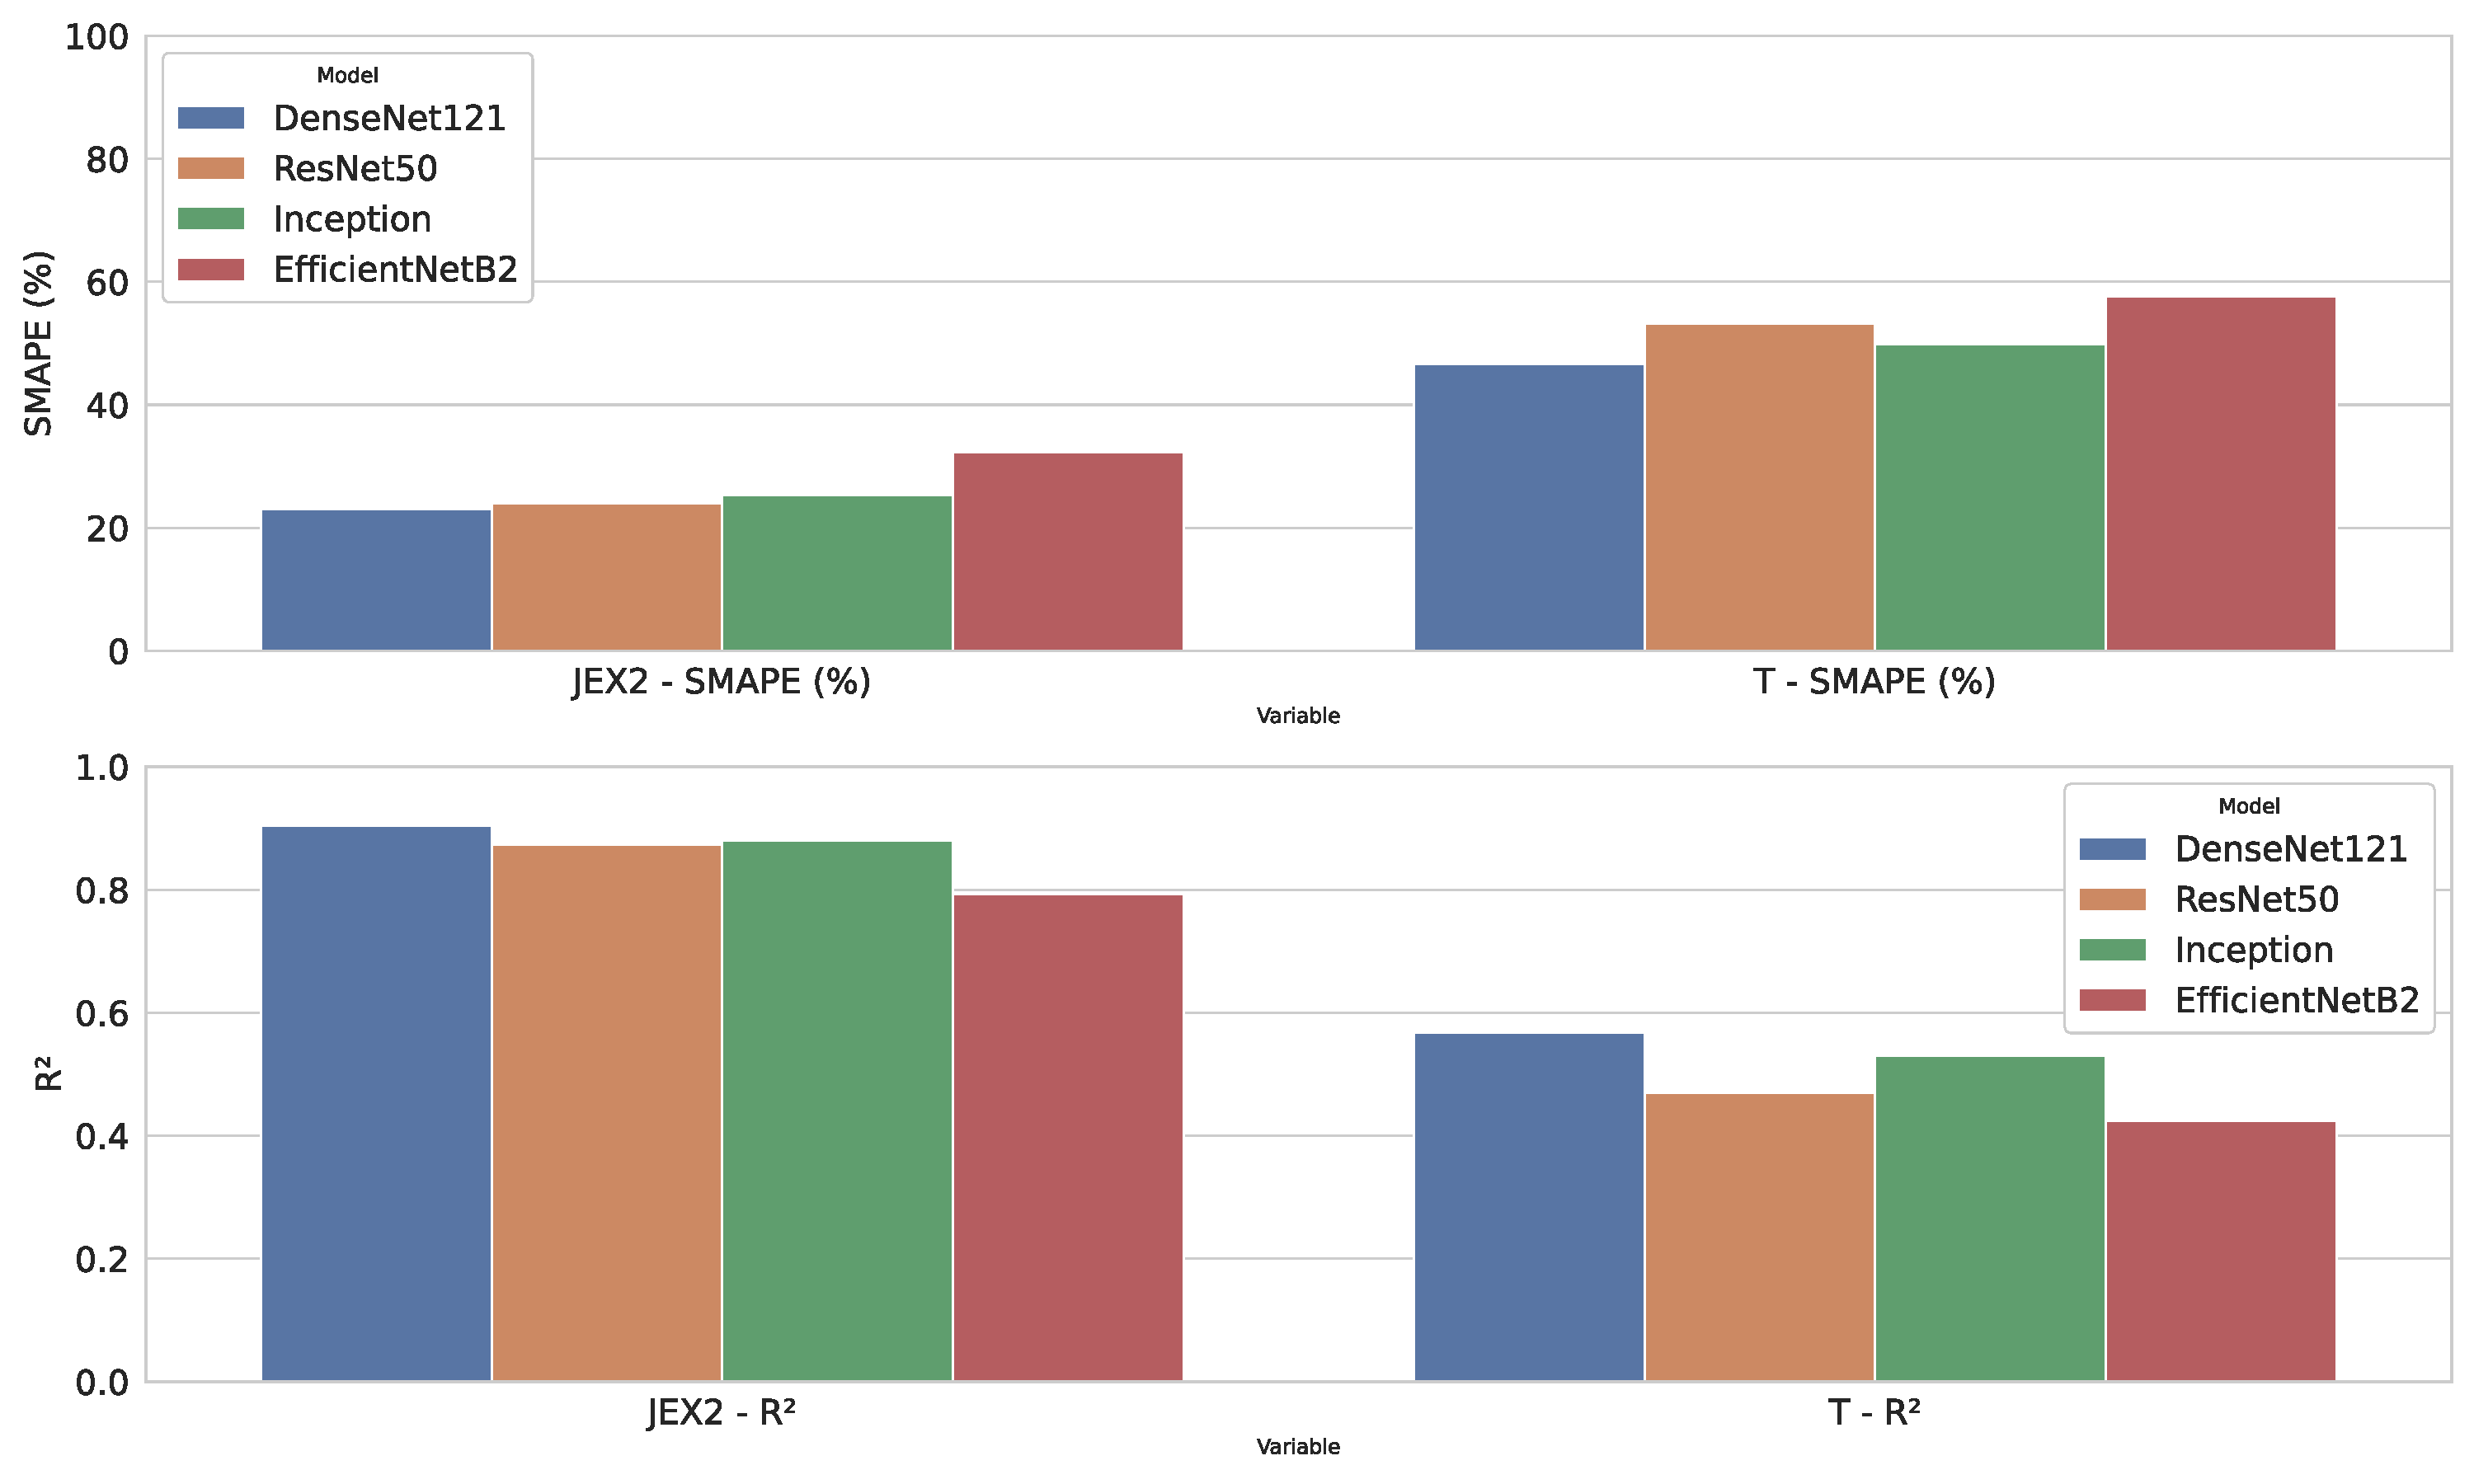
\includegraphics[width=0.95\linewidth]{Figures/comparacion_modelos_separados_JEX2.pdf}
    \caption{Model comparison for the MATERIAL SPINNERS DATA: $R^2$ and SMAPE across architectures for temperature and exchange interaction parameters. Consistent performance trends emerge across datasets.}
    \label{fig:comparison_jex2_inverse}
\end{figure}

Among the evaluated architectures, \textbf{DenseNet121} consistently achieved the best balance across both datasets, exhibiting the lowest SMAPE and highest $R^2$ for the most challenging parameter (KDM). This architecture was therefore selected for further analysis and interpretability studies.

\paragraph{DenseNet Architecture.}
DenseNet (Densely Connected Convolutional Networks) employs a concatenation strategy for layer activations, in contrast to ResNet's additive residual connections. Each layer within a dense block receives as input the concatenated outputs of all preceding layers. This dense connectivity enables efficient feature reuse, reduces the number of parameters, and mitigates the vanishing gradient problem, making DenseNet particularly well-suited for complex regression tasks.

\begin{figure}[H]
\centering
\includegraphics[width=0.9\linewidth]{Figures/Densenet_diagram_V2.png}
\caption{DenseNet121 architecture with dense blocks and transition layers. Feature reuse through concatenation enables parameter efficiency and improved gradient flow.}
\label{fig:densenet_diagram}
\end{figure}

\subsubsection{Experimental Results: KDM DATABASE}

Figure~\ref{fig:densenet_results_kdm} presents the regression results for DenseNet121 on the KDM DATABASE test set. The model achieves accurate predictions for temperature $T$, with minimal scatter around the identity line. However, estimations for $KDM$ exhibit greater dispersion, particularly at intermediate and high values.

\begin{figure}[H]
\centering
\includegraphics[width=0.85\linewidth]{Figures/REGRESION_DENSENET_RESULTS.png}
\caption{DenseNet121 regression results for the KDM DATABASE. Left: temperature estimation shows high fidelity. Right: KDM estimation exhibits increased scatter, especially at higher values.}
\label{fig:densenet_results_kdm}
\end{figure}

This increased dispersion in KDM predictions is primarily attributable to the loss of magnetic order near the Curie temperature. Figure~\ref{fig:kdm_temp_scatter} provides a visual inspection of spin configurations across the KDM parameter space, conditioned on temperature. Coherent magnetic structures are observed for $T < 10$~K, whereas above this threshold, thermal fluctuations dominate and reduce prediction reliability.

\begin{figure}[H]
\centering
\includegraphics[width=0.85\linewidth]{Figures/TvsKDM.png}
\caption{Visual inspection of spin configurations over the KDM parameter space conditioned on temperature. Reliable magnetic structures are observed for $T < 10$~K. Above this range, thermal fluctuations dominate and reduce prediction reliability.}
\label{fig:kdm_temp_scatter}
\end{figure}

To validate this hypothesis, we filtered the test set to include only samples with $T > 10$~K and re-evaluated the model's performance. Figure~\ref{fig:kdm_scatter_high_t} confirms the deterioration in KDM estimation quality in this high-temperature regime, as evidenced by increased deviation from the identity line.

\begin{figure}[H]
\centering
\includegraphics[width=0.75\linewidth]{Figures/KDM_T_ESTIMATIONv2.png}
\caption{DenseNet121 estimation performance for KDM after filtering the test set to include only states with $T > 10$~K. The increased dispersion reflects reduced reliability in the high-temperature regime, where thermal fluctuations disrupt magnetic ordering near the Curie point.}
\label{fig:kdm_scatter_high_t}
\end{figure}

\paragraph{Cross-Dataset Generalization.}
To evaluate the model's ability to generalize across different Hamiltonian formulations, we trained DenseNet121 on the KDM DATABASE SPINERS and tested it on the MATERIAL SPINNERS DATA. The target variable for this cross-dataset evaluation was temperature $T$, as it is the only common varying parameter. This experiment assesses whether the model can capture latent similarities between spin domain configurations even under different physical regimes.

\begin{figure}[H]
\centering
\includegraphics[width=0.75\linewidth]{Figures/Cross.png}
\caption{Cross-dataset evaluation setup: DenseNet121 trained on KDM DATABASE and tested on MATERIAL SPINNERS DATA for temperature estimation. This tests the model's robustness to variations in Hamiltonian parameters.}
\label{fig:cross_dataset}
\end{figure}

\subsubsection{Interpretability via Layer-Wise UMAP Analysis}

To understand how DenseNet121 encodes physical information throughout its layers, we performed a layer-wise analysis using Uniform Manifold Approximation and Projection (UMAP). Intermediate activations were extracted from four representative convolutional layers and projected into 2D embeddings. Each embedding was colored according to either temperature $T$ (Figure~\ref{fig:umap_temp_inverse}) or KDM (Figure~\ref{fig:umap_kdm_inverse}).

\begin{figure}[H]
\centering
\includegraphics[width=0.85\linewidth]{Figures/UMAP_T.png}
\caption{UMAP projections of intermediate activations from DenseNet121, colored by temperature (T). A clear separation emerges in deeper layers, indicating strong internal encoding of thermal behavior.}
\label{fig:umap_temp_inverse}
\end{figure}

\begin{figure}[H]
\centering
\includegraphics[width=0.85\linewidth]{Figures/UMAP_KDM.png}
\caption{UMAP projections of intermediate activations from DenseNet121, colored by Dzyaloshinskii–Moriya interaction (KDM). The representations are less linearly separable, consistent with the increased difficulty in predicting this parameter.}
\label{fig:umap_kdm_inverse}
\end{figure}

These visualizations reveal that deeper layers exhibit progressively more structured separation with respect to $T$, while embeddings colored by $KDM$ show greater variability and complexity. This aligns with the observed regression performance.

To further explore the final latent representation, we extracted activations from the last convolutional layer and overlaid representative spin configuration images at their respective UMAP coordinates (Figure~\ref{fig:latent_space_kdm_inverse}). This composite visualization allows qualitative assessment of how the model clusters similar magnetic states and how these clusters align with variations in KDM.

\begin{figure}[H]
\centering
\includegraphics[width=0.85\linewidth]{Figures/UMAP_IMAGE_KDM.png}
\caption{UMAP projection of the final convolutional layer activations, colored by KDM, with representative spin configuration images overlaid. Smoother color gradients within regions suggest stronger correlation between latent structure and the target variable.}
\label{fig:latent_space_kdm_inverse}
\end{figure}

\subsubsection{Interpretability via Regression Activation Maps (RAMs)}

Following the training phase, we applied \textit{Class Activation Maps (CAMs)} as a post hoc explainability technique to identify the most relevant spatial regions contributing to the regression predictions. For regression tasks, we propose a modified approach termed \textit{Regression Activation Maps (RAMs)}, in which the gradient weighting is defined proportional to prediction accuracy rather than classification confidence:
\begin{equation}
\mathcal{L}_{\text{RAM}} = 1 - \left|y_i - \hat{y}_i\right|.
\end{equation}
This loss is used in gradient-based activation computation, highlighting the spatial regions in the input image that contribute most to accurate predictions.

To examine spatial contribution patterns across different value ranges of KDM, the test dataset was stratified into five groups based on predefined KDM intervals (Figure~\ref{fig:kdm_ranges}). RAMs were computed for representative samples within each group.

\begin{figure}[H]
\centering
\includegraphics[width=0.8\linewidth]{Figures/Ranges.png}
\caption{Stratification of the KDM parameter space into five ranges for interpretability analysis via Regression Activation Maps.}
\label{fig:kdm_ranges}
\end{figure}

Figure~\ref{fig:ram_activation} presents the activation maps for representative magnetic domain states across the five KDM ranges. These visualizations reveal that the model adaptively focuses on different spatial features depending on the KDM value, with increased attention to domain wall structures and topological defects in higher KDM regimes.

\begin{figure}[H]
    \centering
    \includegraphics[width=0.85\linewidth]{Figures/gradcam_1.pdf}
    \caption{Regression Activation Maps (RAMs) for magnetic domain states across five KDM ranges. The model's attention shifts toward domain walls and topological features as KDM increases.}
    \label{fig:ram_activation}
\end{figure}

\paragraph{Layer-Level Cumulative Analysis.}
To quantify the contribution of each convolutional layer to the regression task across different KDM ranges, we computed the cumulative activation of RAMs per layer and per KDM value group. For each of the five KDM ranges, we aggregated the activation maps across all test images belonging to that range. Figure~\ref{fig:ram_cumulative} presents this layer-wise cumulative analysis, revealing which stages of the network architecture are most sensitive or informative for predicting low, medium, and high KDM values.

\begin{figure}[H]
    \centering
    \includegraphics[width=0.85\linewidth]{Figures/mean_contribution_gradcam2.pdf}
    \caption{Cumulative activation maps per convolutional layer across five predefined KDM value ranges. Different layers exhibit varying sensitivity to specific KDM regimes, providing layer-level interpretability.}
    \label{fig:ram_cumulative}
\end{figure}

\paragraph{Discussion.}
This proof-of-concept demonstrates that transfer learning-based CNNs can effectively solve the inverse problem of parameter estimation from magnetic domain images. Key findings include:
\begin{itemize}
    \item \textbf{Architecture Selection}: DenseNet121 achieves the best balance across datasets and target variables, with particularly strong performance for temperature estimation.
    \item \textbf{Parameter-Specific Challenges}: KDM estimation is inherently more difficult than temperature estimation, particularly in high-temperature regimes where thermal disorder dominates.
    \item \textbf{Cross-Dataset Generalization}: The model trained on one Hamiltonian formulation can generalize to predict temperature in a different physical regime, suggesting that latent representations capture transferable magnetic features.
    \item \textbf{Interpretability}: UMAP analysis reveals that deeper layers progressively organize representations according to physical parameters, while RAMs provide spatial interpretability, highlighting which regions of the magnetic configuration contribute most to accurate predictions.
\end{itemize}

These results establish a baseline for inverse parameter estimation and motivate future integration with the forward generative pipeline (cVAE) into a unified bidirectional framework capable of both state generation and parameter inference.


\section{Conclusions} \label{sec:Conclusions}

This work proposes a physics-informed deep learning framework to address three fundamental challenges in nanoscale magnetic domain characterization: parameter degeneracy, data quality degradation, and lack of interpretability. The methodology integrates conditional generative modeling with learned physics-guided priors, inverse parameter estimation via transfer learning, cycle-consistency constraints, physics-based regularization, and domain adaptation strategies to bridge synthetic and experimental data.

Two proof-of-concept studies validate the feasibility of the core components using large-scale Monte Carlo datasets totaling over 200,000 magnetic domain images. The conditional VAE demonstrates that parameter-conditioned latent priors can organize representations according to physical parameters even without explicit energy constraints, achieving high-fidelity reconstructions of complex magnetic textures. The inverse problem study confirms that transfer learning-based CNNs (particularly DenseNet121) can effectively estimate Hamiltonian parameters from spin configurations, with strong performance for temperature prediction and challenges for Dzyaloshinskii–Moriya interaction estimation in high-disorder regimes. Layer-wise interpretability analysis via UMAP and the novel Regression Activation Maps methodology reveals that deeper network layers progressively encode physical information and adaptively focus on topologically relevant features.

Critical limitations have been identified that guide the next development phase. Hyperparameter optimization via Bayesian methods is required to fully exploit model capacity. More fundamentally, the geometric invariance of magnetic configurations necessitates evaluation metrics beyond pixel-level comparisons—future work must incorporate rotation-invariant topological descriptors, energy-based metrics, and perceptual similarity measures adapted to magnetic textures.

The path forward involves integrating the validated forward and inverse pipelines into a unified cycle-consistent framework, incorporating micromagnetic energy penalties and Landau-Lifshitz-Gilbert residuals to enforce strict physical constraints, and developing domain adaptation strategies to transfer knowledge from high-fidelity simulations to experimental microscopy data. The proof-of-concept results establish a promising foundation for physics-informed deep learning in this domain, demonstrating that the proposed components can address degeneracy, enhance generative quality, and provide interpretability while revealing critical methodological refinements needed for robust deployment in experimental scenarios.


\section{Future Work}\label{sec:future_work}

The proof-of-concept results presented in this work establish the foundation for several critical research directions that will consolidate the proposed physics-informed framework into a robust and deployable system for nanoscale magnetic domain characterization.

\paragraph{Hyperparameter Optimization and Model Refinement.}
Systematic Bayesian optimization using frameworks such as Optuna will be conducted to identify optimal configurations for the conditional VAE and inverse estimation architectures. This includes tuning the $\beta$ parameter in the loss function, latent space dimensionality, learning rates, network depth, and prior network capacity. Preliminary experiments used manually selected hyperparameters; rigorous optimization is expected to significantly enhance both generative quality and parameter estimation accuracy.

\paragraph{Integration of Forward and Inverse Pipelines.}
The next critical step involves unifying the forward generative pathway (cVAE) and inverse estimation pathway (DenseNet-based regressor) into a single cycle-consistent framework. This integration will enable the enforcement of bidirectional constraints: generated configurations must yield consistent parameter estimates when passed through the inverse model, and estimated parameters must regenerate configurations similar to the original inputs. This cycle-consistency regularization ($\mathcal{L}_{\text{cycle}}$) is expected to substantially reduce parameter degeneracy and improve physical identifiability, particularly for challenging parameters such as the Dzyaloshinskii–Moriya interaction in high-temperature regimes.

\paragraph{Physics-Informed Regularization.}
Explicit incorporation of micromagnetic energy functionals (exchange, anisotropy, Zeeman, and DMI contributions) and Landau-Lifshitz-Gilbert residuals into the loss function will enforce strict adherence to fundamental physical constraints. These physics-based penalties ($\mathcal{L}_{\text{energy}}$ and $\mathcal{L}_{\text{LLG}}$) will ensure that generated magnetic configurations are not only visually plausible but also energetically stable and dynamically consistent with micromagnetic theory. This is particularly critical for generalization to unseen parameter regimes and for robustness to out-of-distribution inputs.

\paragraph{Handling Low-Quality Data and Domain Adaptation.}
Addressing the degradation of experimental magnetic domain images requires developing robust domain adaptation strategies to transfer knowledge from high-fidelity Monte Carlo simulations to noisy, artifact-laden experimental data from MFM and LTEM microscopy. Adversarial domain adaptation techniques, including domain-adversarial neural networks (DANN) and adversarial discriminative domain adaptation (ADDA), will be explored to align latent representations across synthetic and experimental domains. Additionally, generative adversarial networks (GANs) and self-supervised denoising methods (e.g., Noise2Void) will be investigated for image quality enhancement while preserving physical structure. These techniques must be carefully validated to ensure that noise removal does not introduce spurious magnetic features or suppress genuine physical variability.

\paragraph{Evaluation Metrics and Interpretability.}
The geometric invariance of magnetic configurations necessitates the development of evaluation metrics beyond pixel-level comparisons. Future work will implement rotation- and translation-invariant topological descriptors (e.g., skyrmion number, vortex core counting, domain wall density), energy-based metrics computed from micromagnetic Hamiltonians, and perceptual similarity measures adapted to magnetic textures. Additionally, the Regression Activation Maps (RAMs) methodology introduced in this work will be extended and systematically compared with other interpretability techniques to ensure that model predictions align with physically meaningful features across diverse magnetic regimes.

\paragraph{Comparative Evaluation with Alternative Architectures.}
While this work focuses on conditional variational autoencoders and CNN-based inverse models, emerging generative architectures warrant systematic comparison. Diffusion models, which have demonstrated state-of-the-art performance in image synthesis tasks, offer an alternative generative paradigm with potentially superior sample quality and mode coverage. Similarly, transformer-based architectures have shown promise in capturing long-range dependencies and may provide advantages for modeling extended magnetic domain structures. Future work will conduct controlled comparisons between cVAEs, diffusion models, and transformer-based generators on the same benchmark datasets, evaluating trade-offs in generation quality, parameter efficiency, training stability, and interpretability.

\paragraph{Extension to Experimental Validation and Complex Systems.}
The ultimate validation of the proposed framework requires deployment on real experimental data and extension to more complex magnetic systems. Collaborations with experimental groups will enable access to high-resolution MFM and LTEM datasets, facilitating rigorous testing of the domain adaptation strategies. Furthermore, the methodology will be extended to three-dimensional magnetic nanostructures, multilayer thin films, and systems exhibiting more complex topological textures such as antiskyrmions, skyrmion lattices, and magnetic hopfions. These extensions will test the generality and scalability of the physics-informed deep learning approach across diverse material systems and experimental conditions.


\bibliographystyle{unsrt}
\small{
\bibliography{references}}

\end{document}


